\subsection{Detailed analysis of observation types per navigation signal for Galileo}%
\label{subsec:DetailedanalysisofobservationtypespernavigationsignalforGalileo}%
\setlength{\tabcolsep}{4pt}%
\begin{longtabu}[c]{rcl}%
Observation tabular file&:&TURX00BEL\_R\_20203491400\_30M\_01S\_MO\_E.obstab\\%
Examined satellites&:&E02, E03, E05, E07, E08, E24, E25, E26, E28\\%
Examined navigation signals&:&6A, 1A\\%
Examined observables&:&S1A, S6A\\%
\end{longtabu}%
\subsubsection{TLE time spans}%
\label{ssubsec:TLEtimespans}%
The table below represents the calculated rise and set times within the observation time span for a PRN based on the TLEs. When a culmination is within this interval, it is represented in the table.%
\setlength{\tabcolsep}{4pt}%
\begin{longtabu}[c]{l|l|l|l|c}%
\hline%
\textbf{PRN}&\textbf{tle\_rise}&\textbf{tle\_set}&\textbf{tle\_cul}&\textbf{tle\_arc\_count}\\%
\hline%
\endhead%
\hline%
\multicolumn{5}{r}{Continued on Next Page}\\%
\hline%
\endfoot%
\hline%
\endlastfoot%
E02&14:00:00&14:30:00&&1800.0\\%
E03&14:00:00&14:30:00&&1800.0\\%
E05&14:00:00&14:30:00&&1800.0\\%
E08&14:00:00&14:30:00&&1800.0\\%
E24&14:00:00&14:30:00&&1800.0\\%
E25&14:00:00&14:30:00&14:17:38&1800.0\\%
E26&14:00:00&14:30:00&&1800.0\\%
E28&14:00:00&14:30:00&&1800.0\\%
E07&14:18:50&14:30:00&&670.0\\%
\hline%
\end{longtabu}

%
\subsubsection{Navigation signals analysis for Galileo}%
\label{ssubsec:NavigationsignalsanalysisforGalileo}%
\newpage%
\paragraph{Analysis of navigation signal E6A}%
\label{para:AnalysisofnavigationsignalE6A}%
\begin{enumerate}%
\item%
Figure \ref{fig:tle_navsig_6AE} represents the observed time span for navigation signal E6A set out against the maximum time span calculated from the  Two Line Elements (TLE). If present, the culmination point for a satellite is represented by a triangle. The time span from TLEs is represented by the lighter area while the real observations are represented by the dark super-imposed areas.%


\begin{figure}[H]%
\centering%
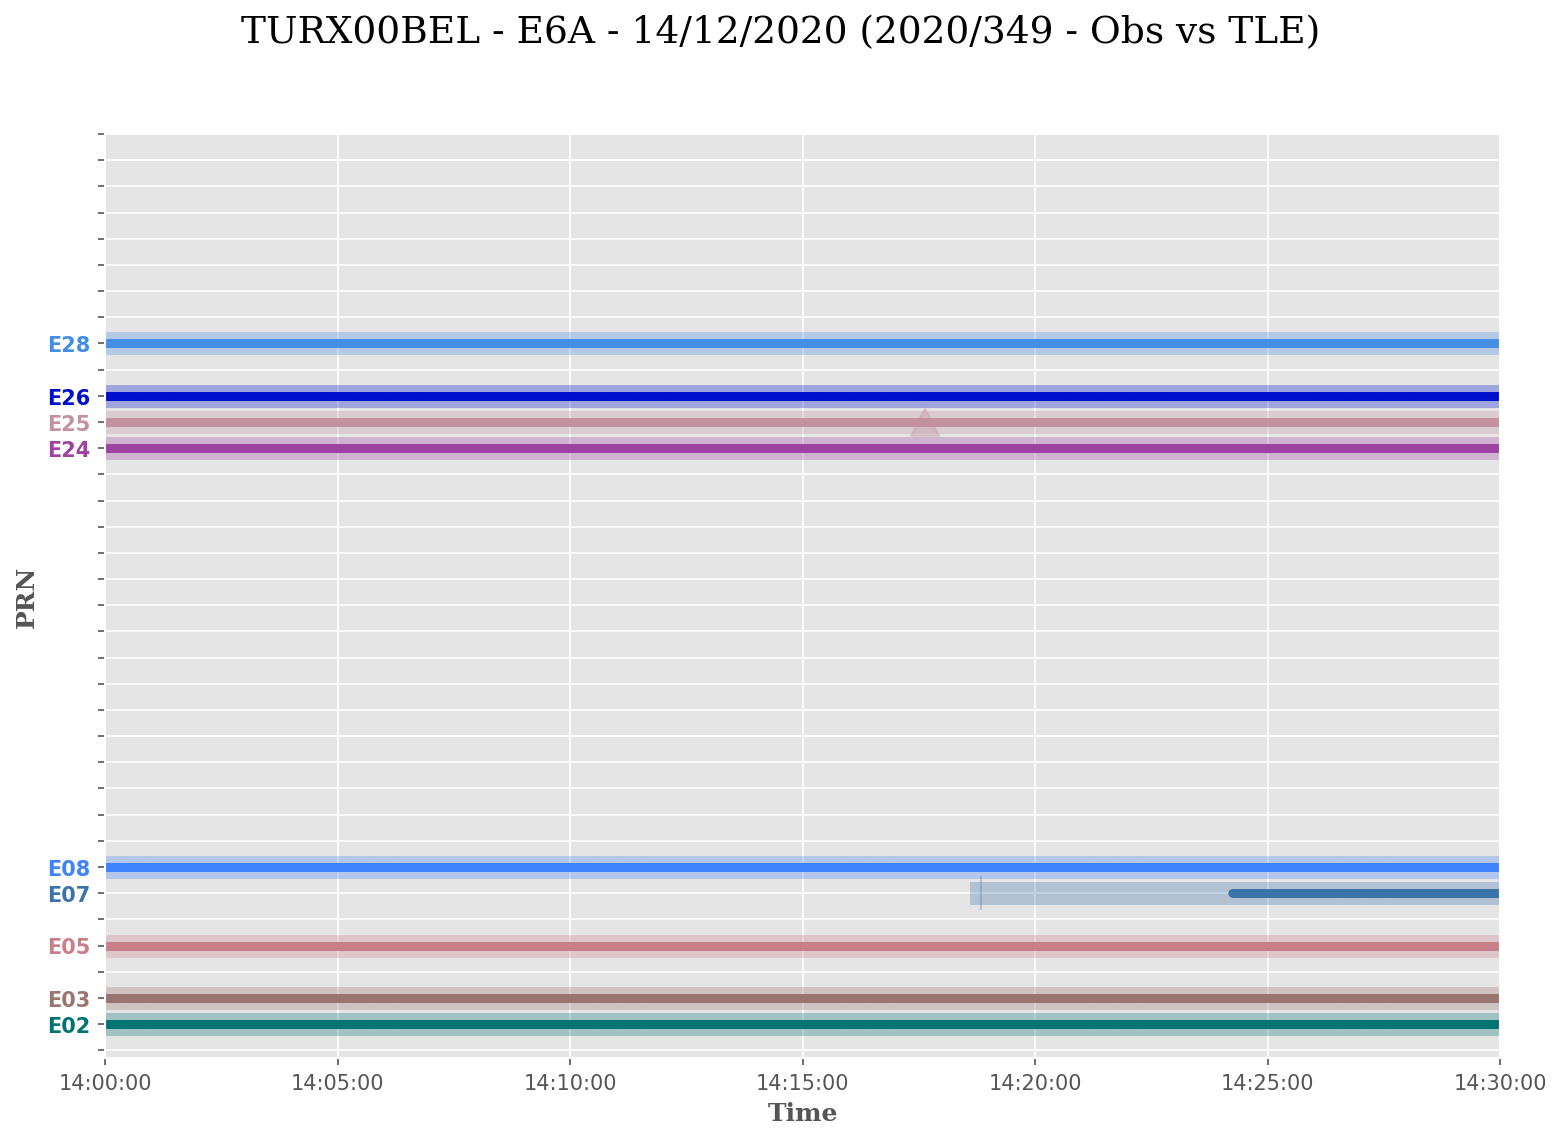
\includegraphics[width=0.95\textwidth]{png/TURX00BEL_R_20203491400_30M_01S_MO_E-E6A-TLE-arcs.png}%
\caption{\label{fig:tle_navsig_6AE} Navigation signal E6A versus TLE time span}%
\end{figure}

%
\item%
Figure \ref{fig:tle_navsig_ES6A} displays the evolution of observation type S6A. \newline The upper plot represents the variation of the observation type while the middle plot (if available) displays the variation of this observable between 2 consecutive epochs. The bottom plot displays the TLE time spans for the satellies.%


\begin{figure}[H]%
\centering%
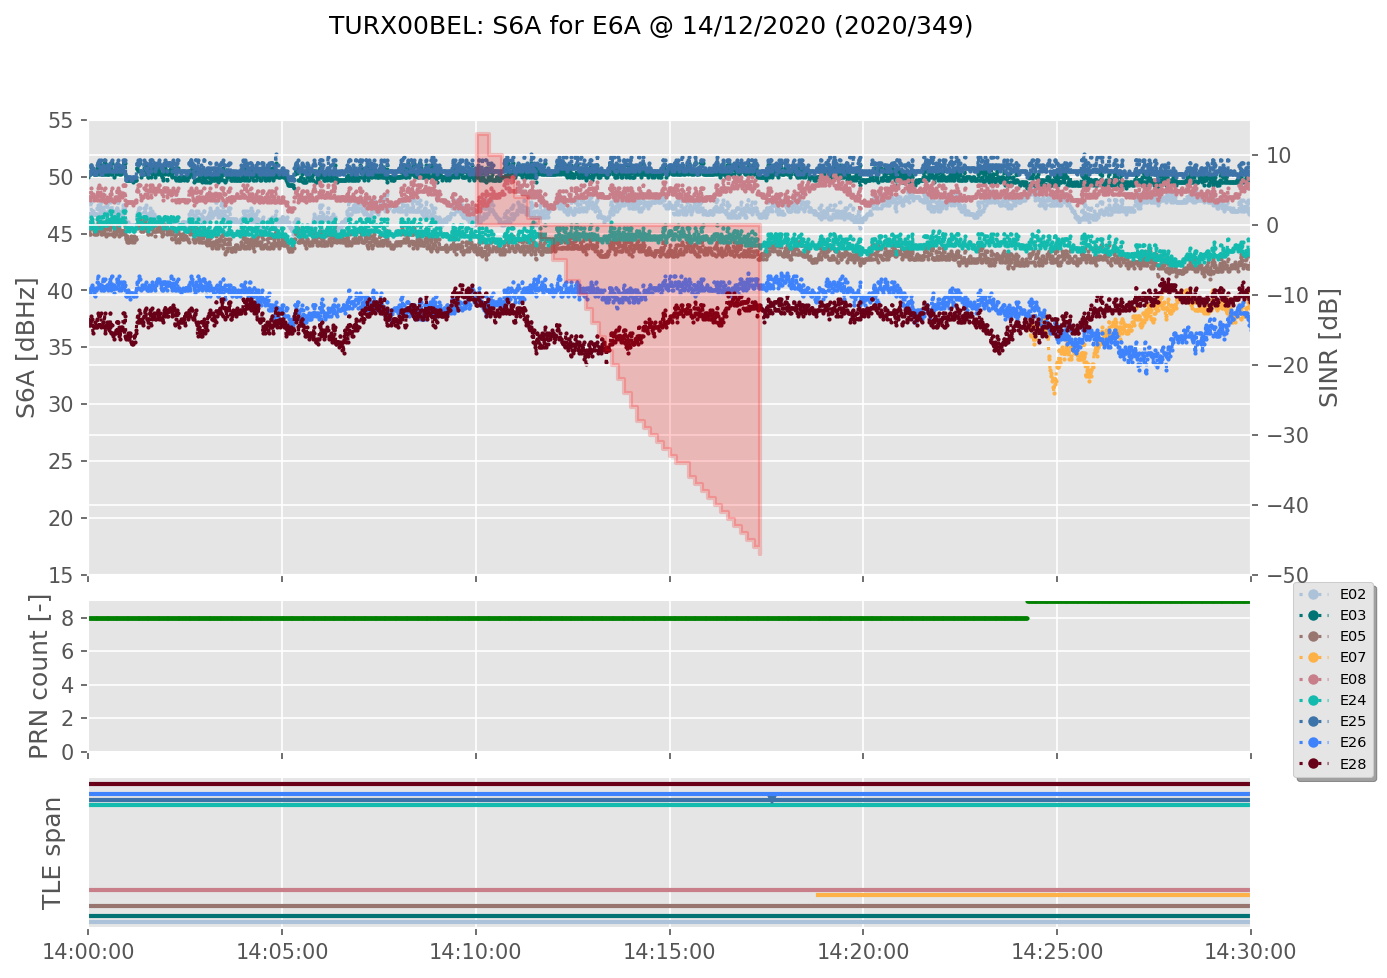
\includegraphics[width=0.95\textwidth]{png/TURX00BEL_R_20203491400_30M_01S_MO_E-E6A-S6A.png}%
\caption{\label{fig:tle_navsig_ES6A} Navigation signal S6A evolution}%
\end{figure}

%
\item%
Analysis of navigation signal E6A for each observed satellite.\newline%
ewline The following plots display the same information as described above per satellite. Each plot is accompanied by a table displaying the time of loss of lock and reacquisition of the satellite when such events are detected.%


\begin{figure}[H]%
\centering%
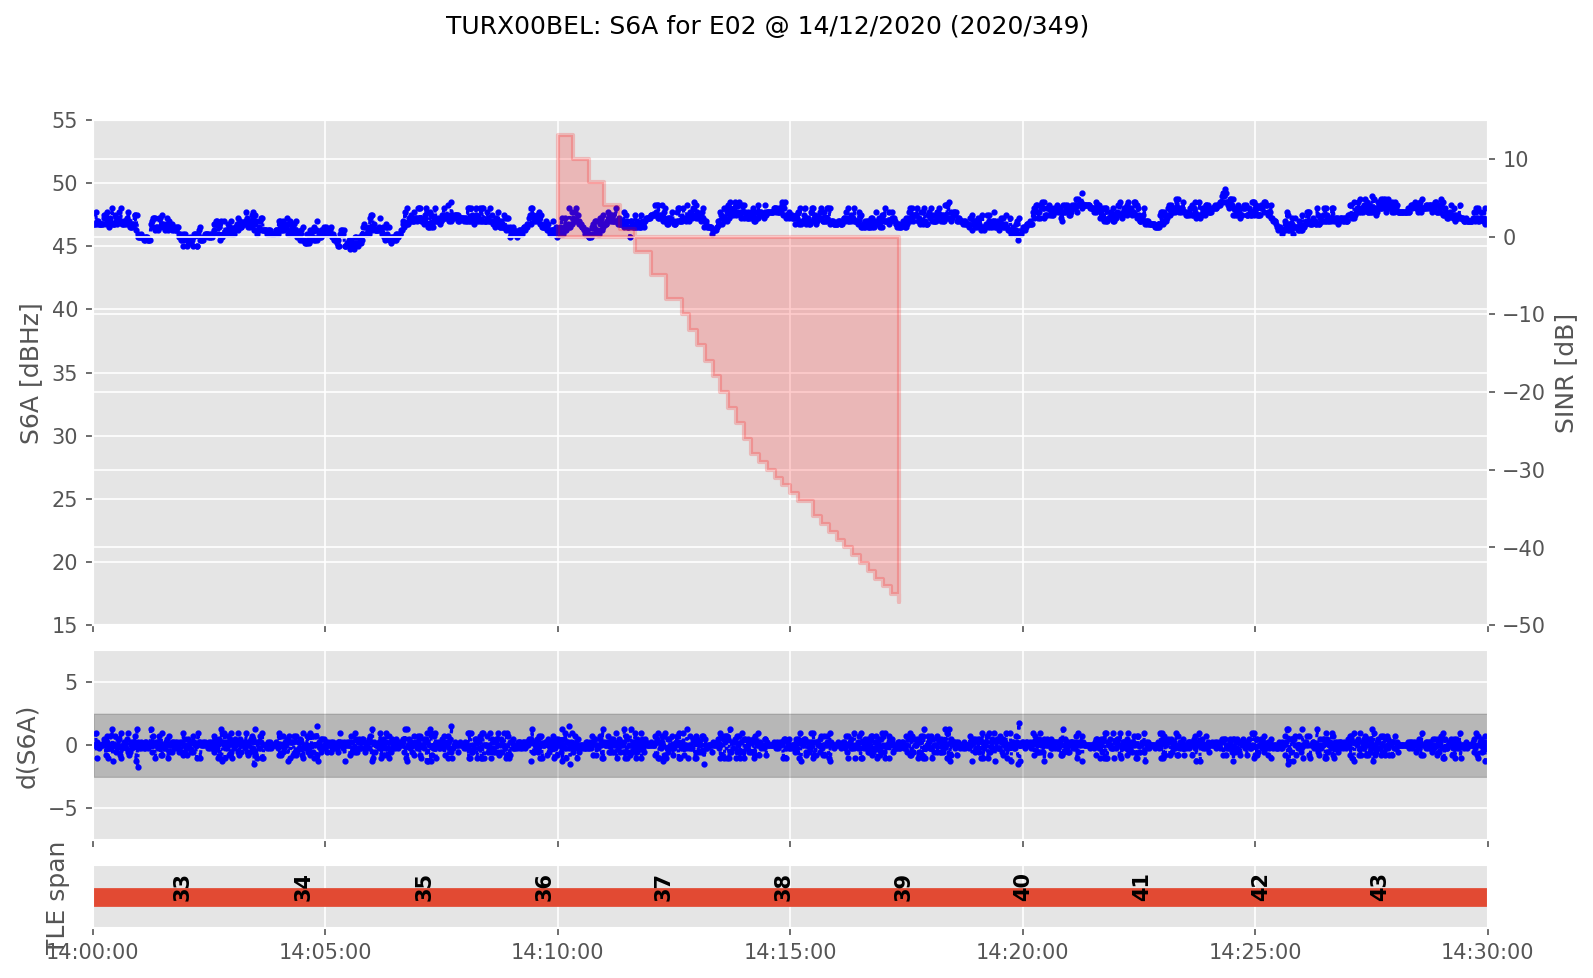
\includegraphics[width=0.95\linewidth]{png/TURX00BEL_R_20203491400_30M_01S_MO_E-S6A-E02.png}%
\end{figure}

%


\begin{figure}[H]%
\centering%
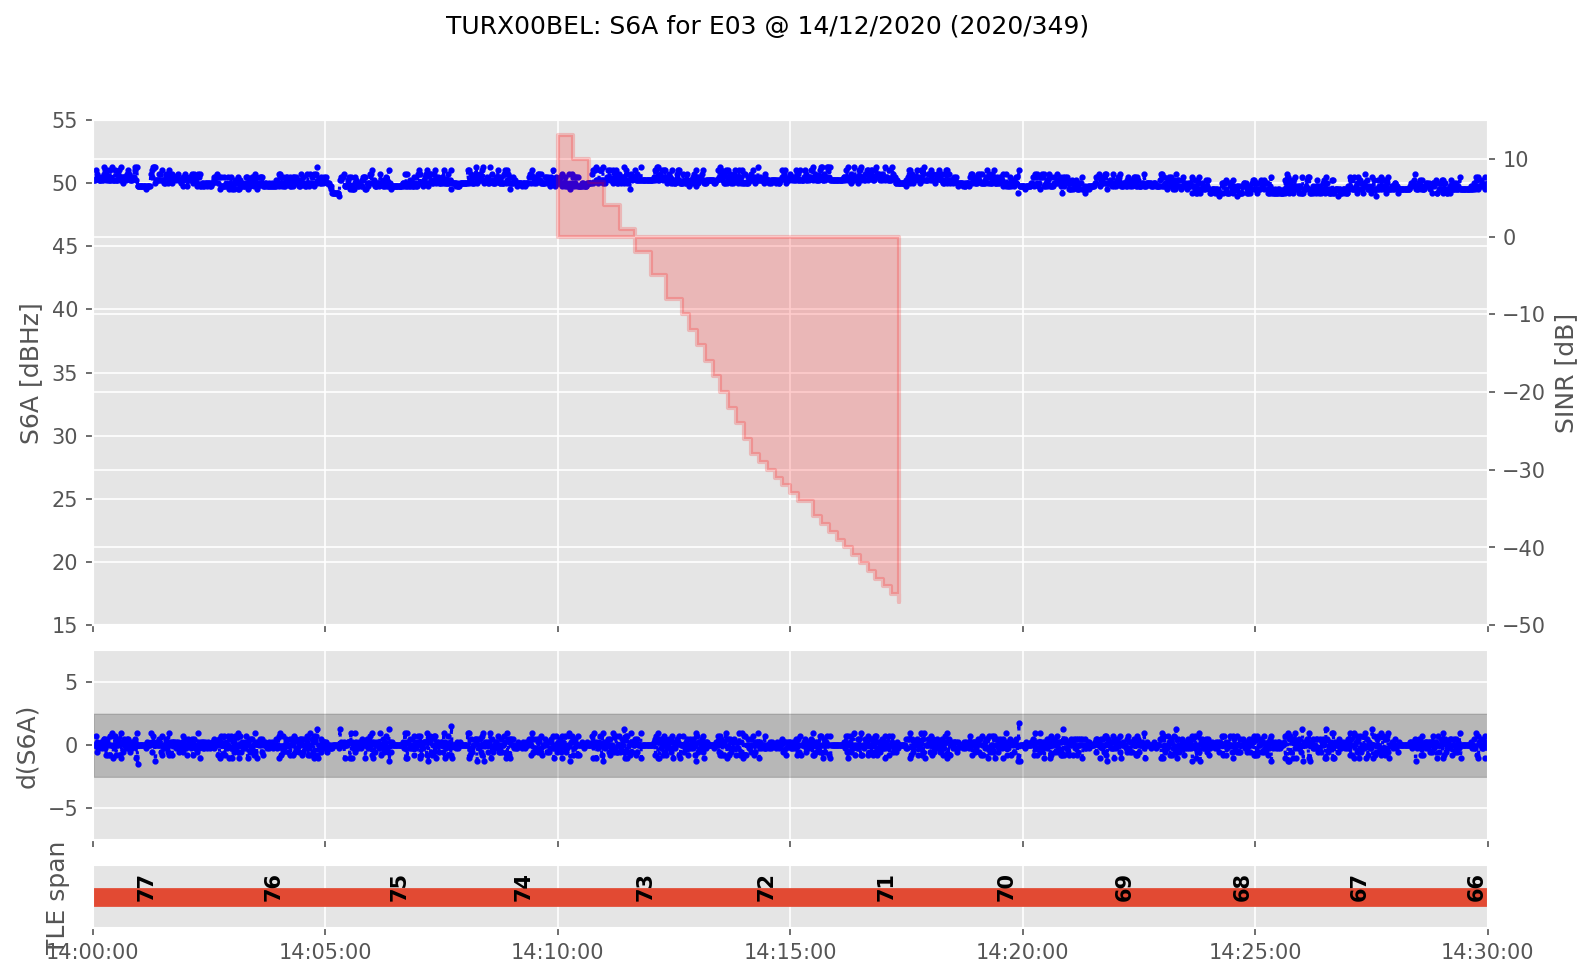
\includegraphics[width=0.95\linewidth]{png/TURX00BEL_R_20203491400_30M_01S_MO_E-S6A-E03.png}%
\end{figure}

%


\begin{figure}[H]%
\centering%
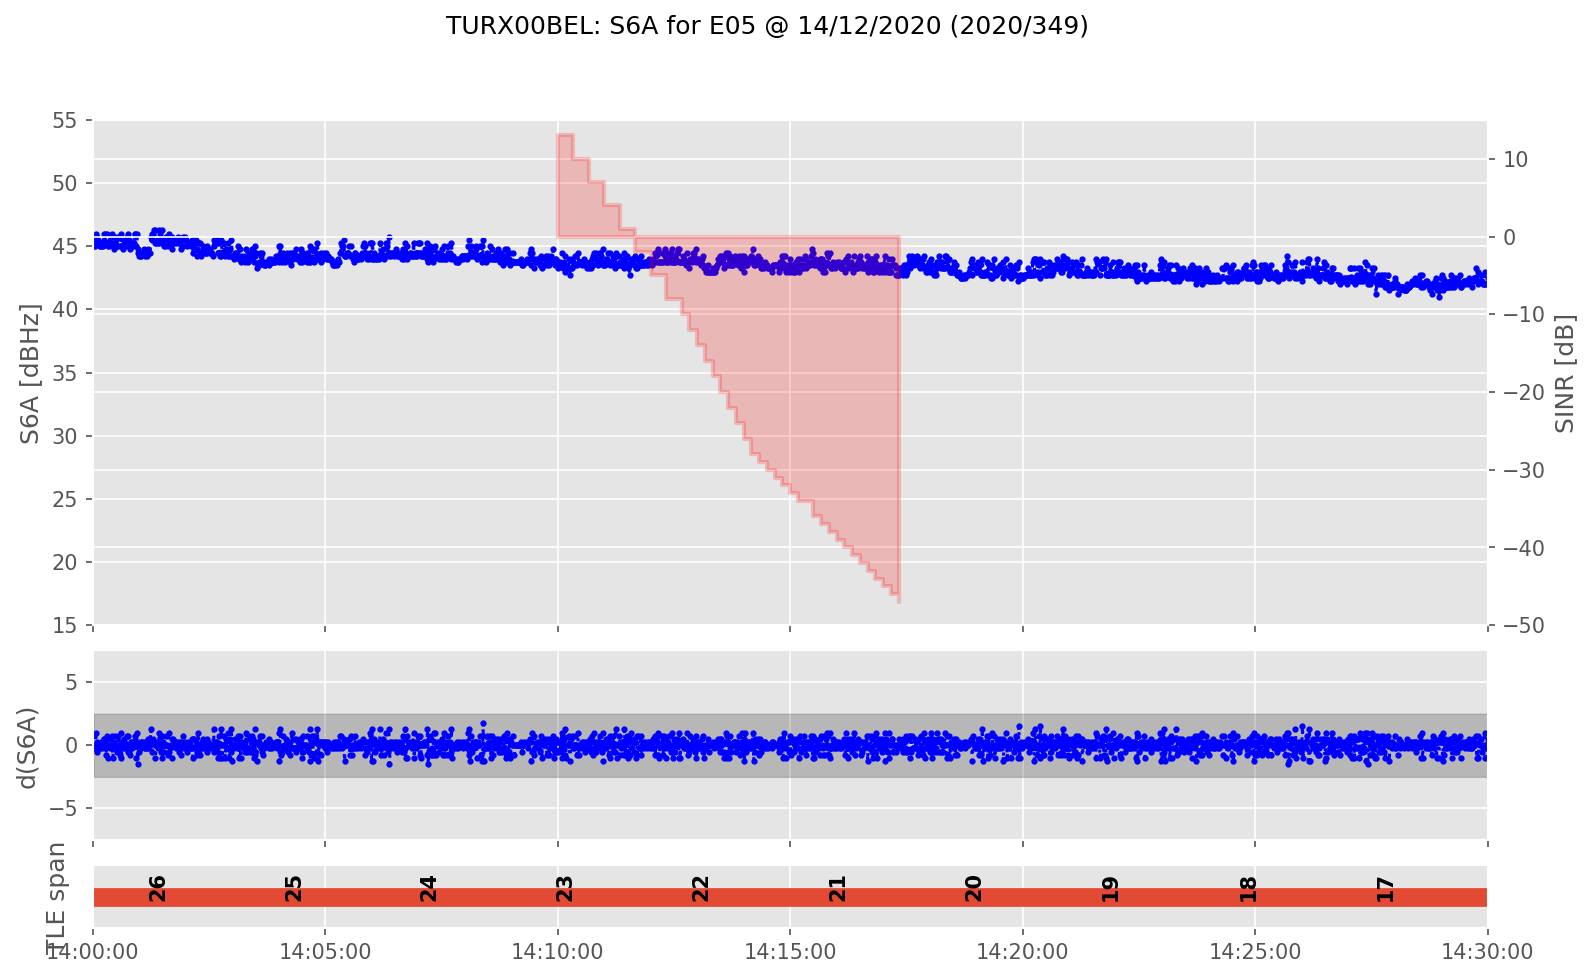
\includegraphics[width=0.95\linewidth]{png/TURX00BEL_R_20203491400_30M_01S_MO_E-S6A-E05.png}%
\end{figure}

%


\begin{figure}[H]%
\centering%
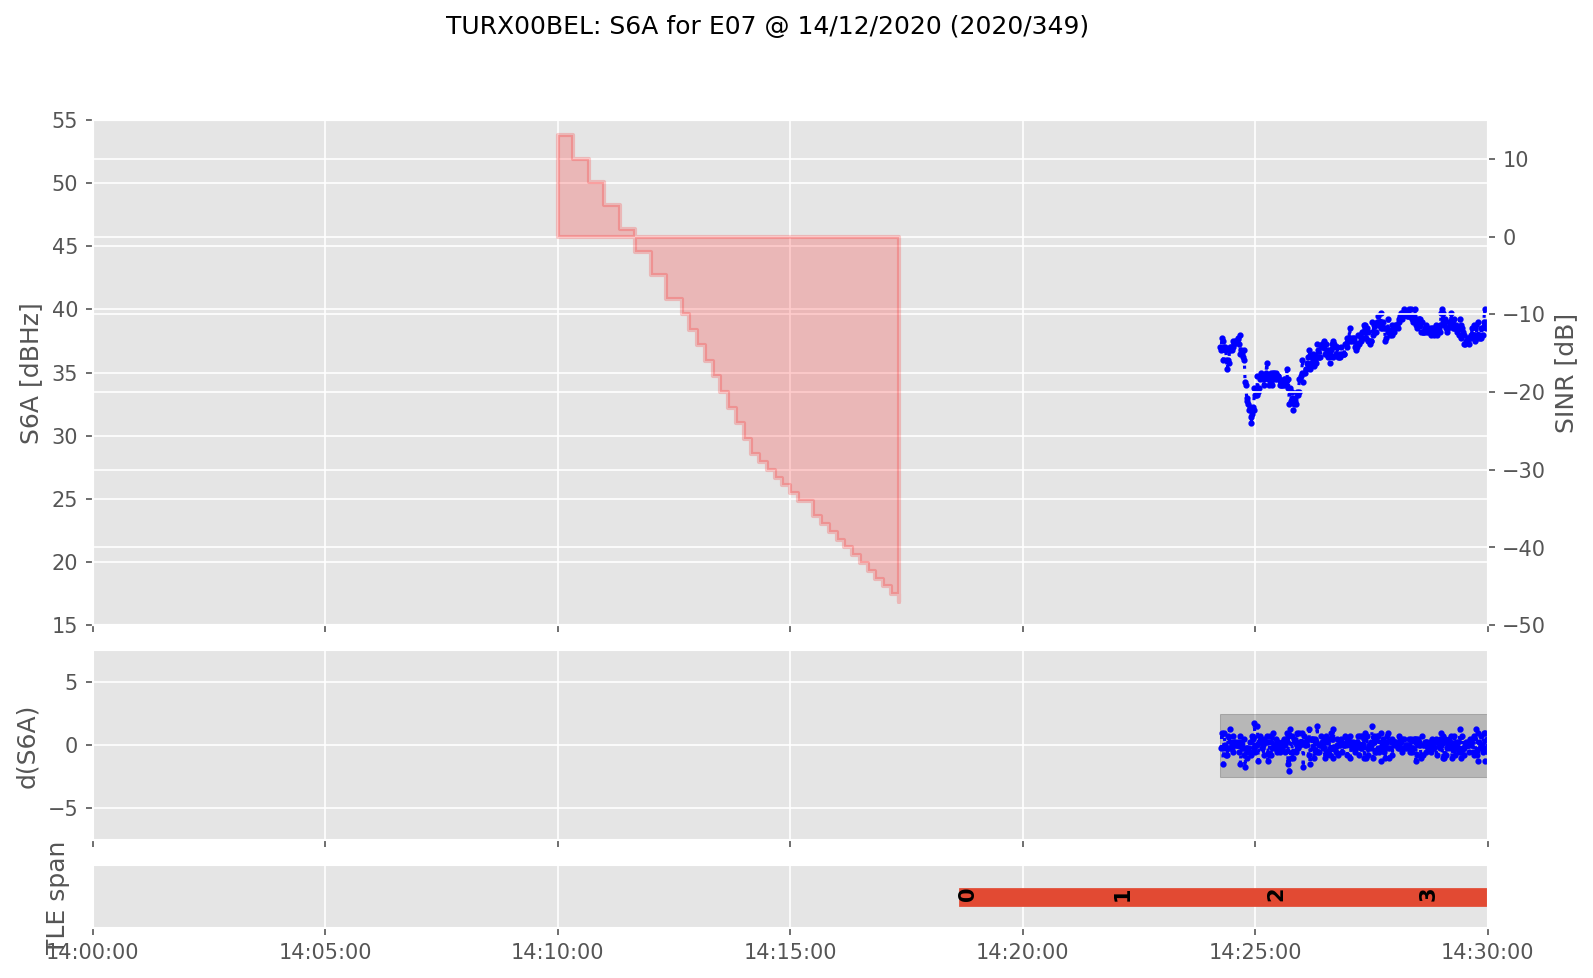
\includegraphics[width=0.95\linewidth]{png/TURX00BEL_R_20203491400_30M_01S_MO_E-S6A-E07.png}%
\end{figure}

%


\begin{figure}[H]%
\centering%
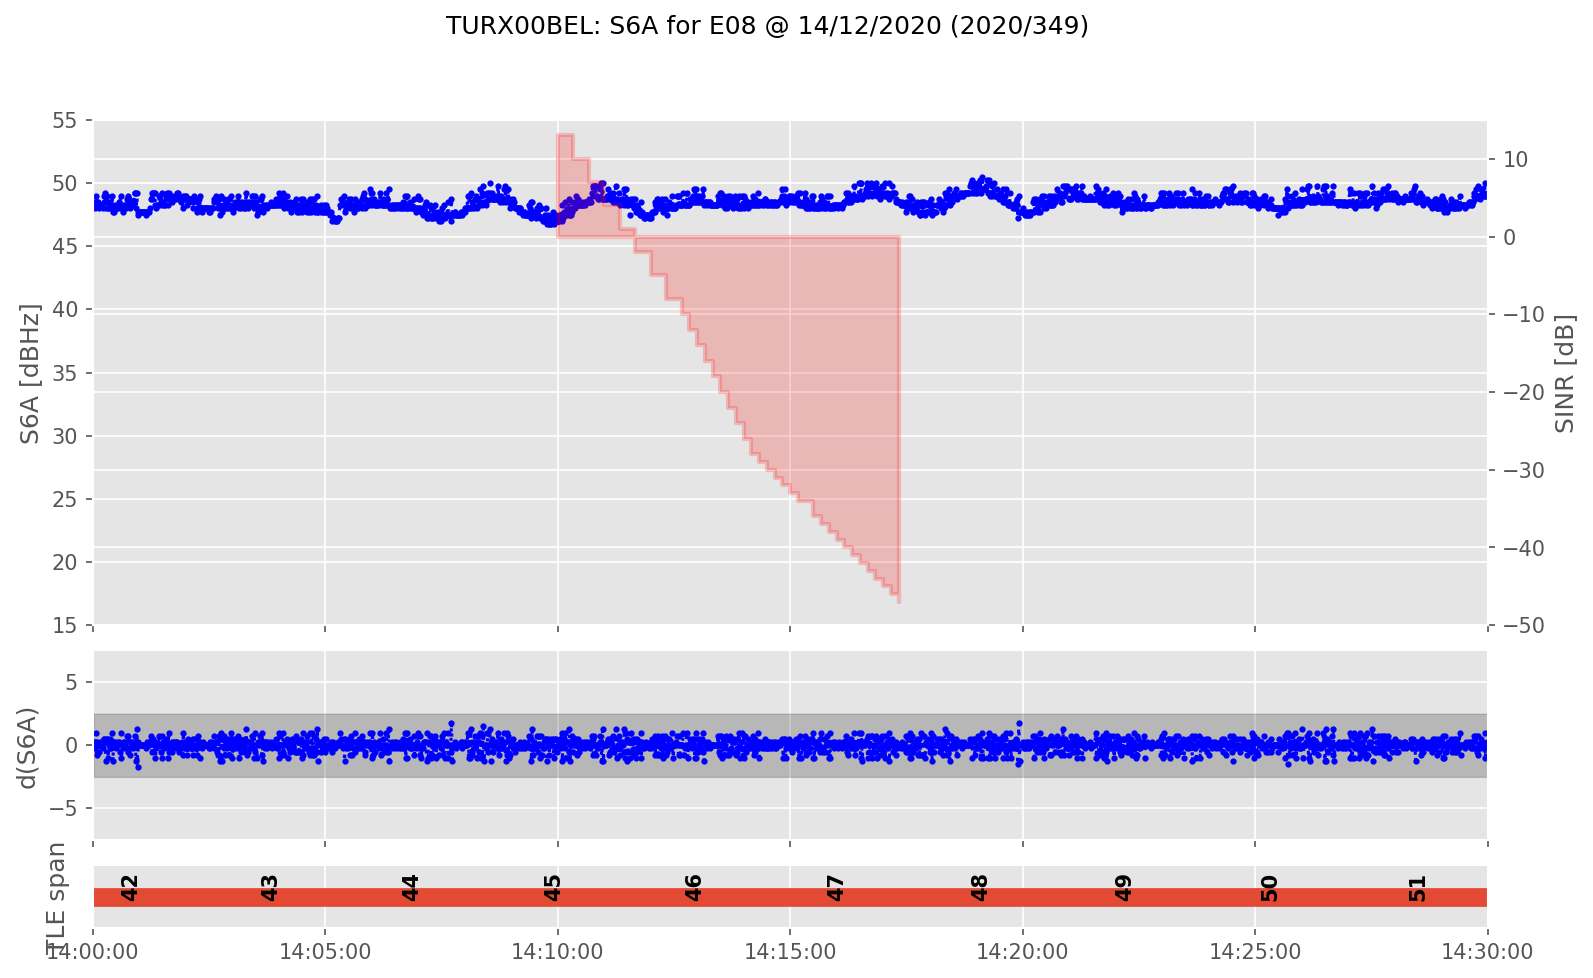
\includegraphics[width=0.95\linewidth]{png/TURX00BEL_R_20203491400_30M_01S_MO_E-S6A-E08.png}%
\end{figure}

%


\begin{figure}[H]%
\centering%
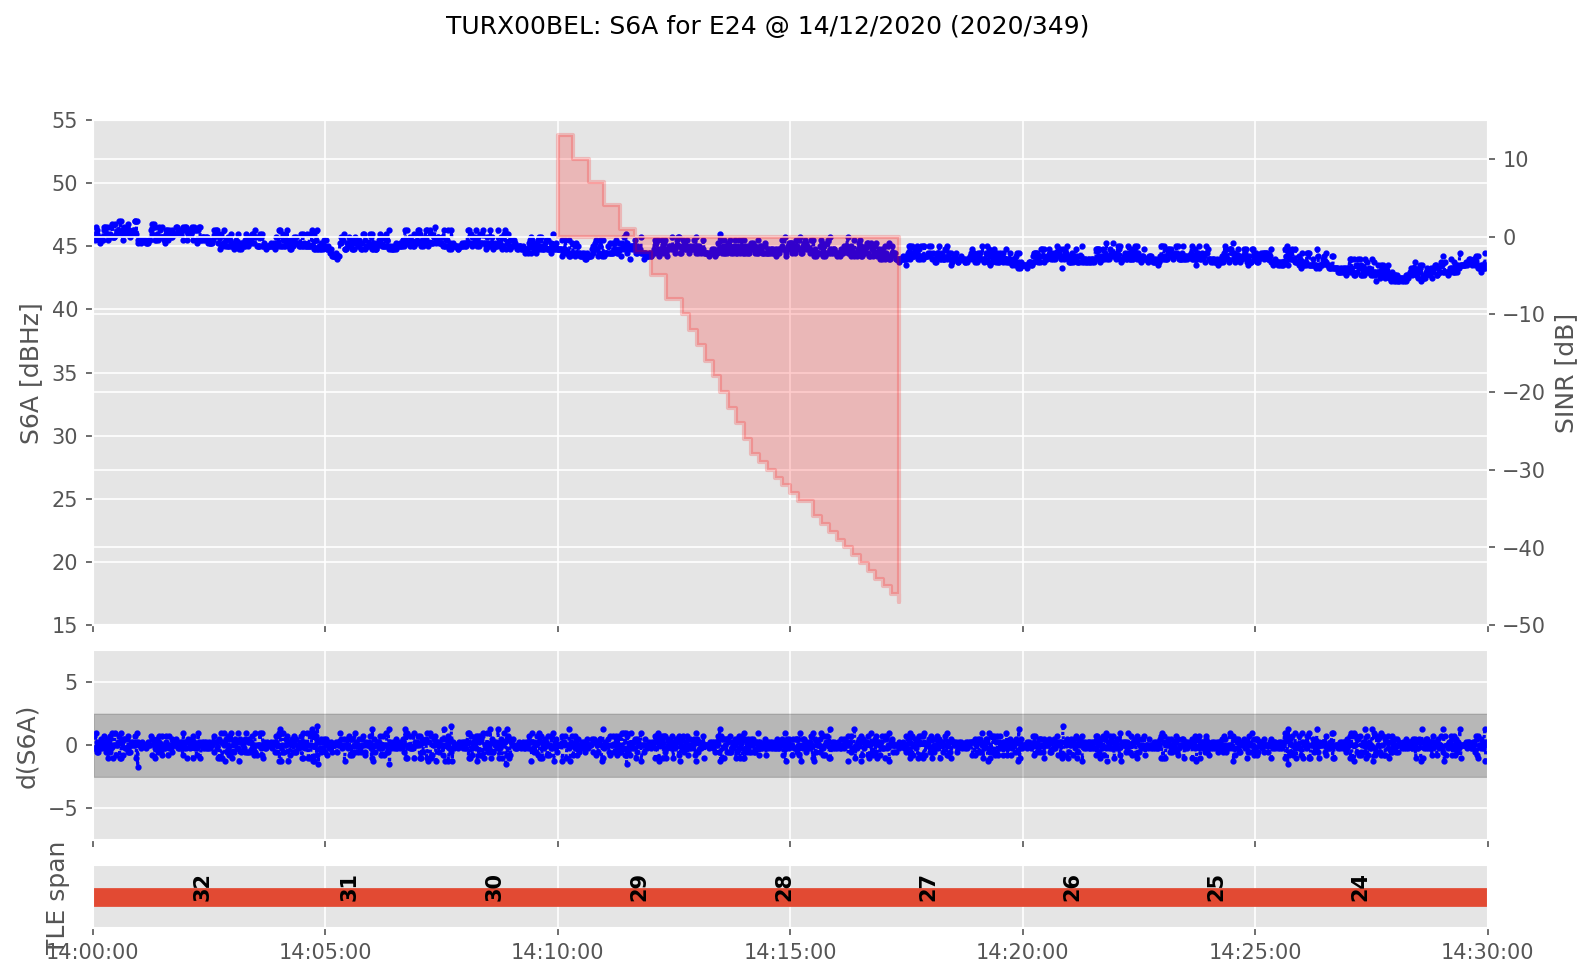
\includegraphics[width=0.95\linewidth]{png/TURX00BEL_R_20203491400_30M_01S_MO_E-S6A-E24.png}%
\end{figure}

%


\begin{figure}[H]%
\centering%
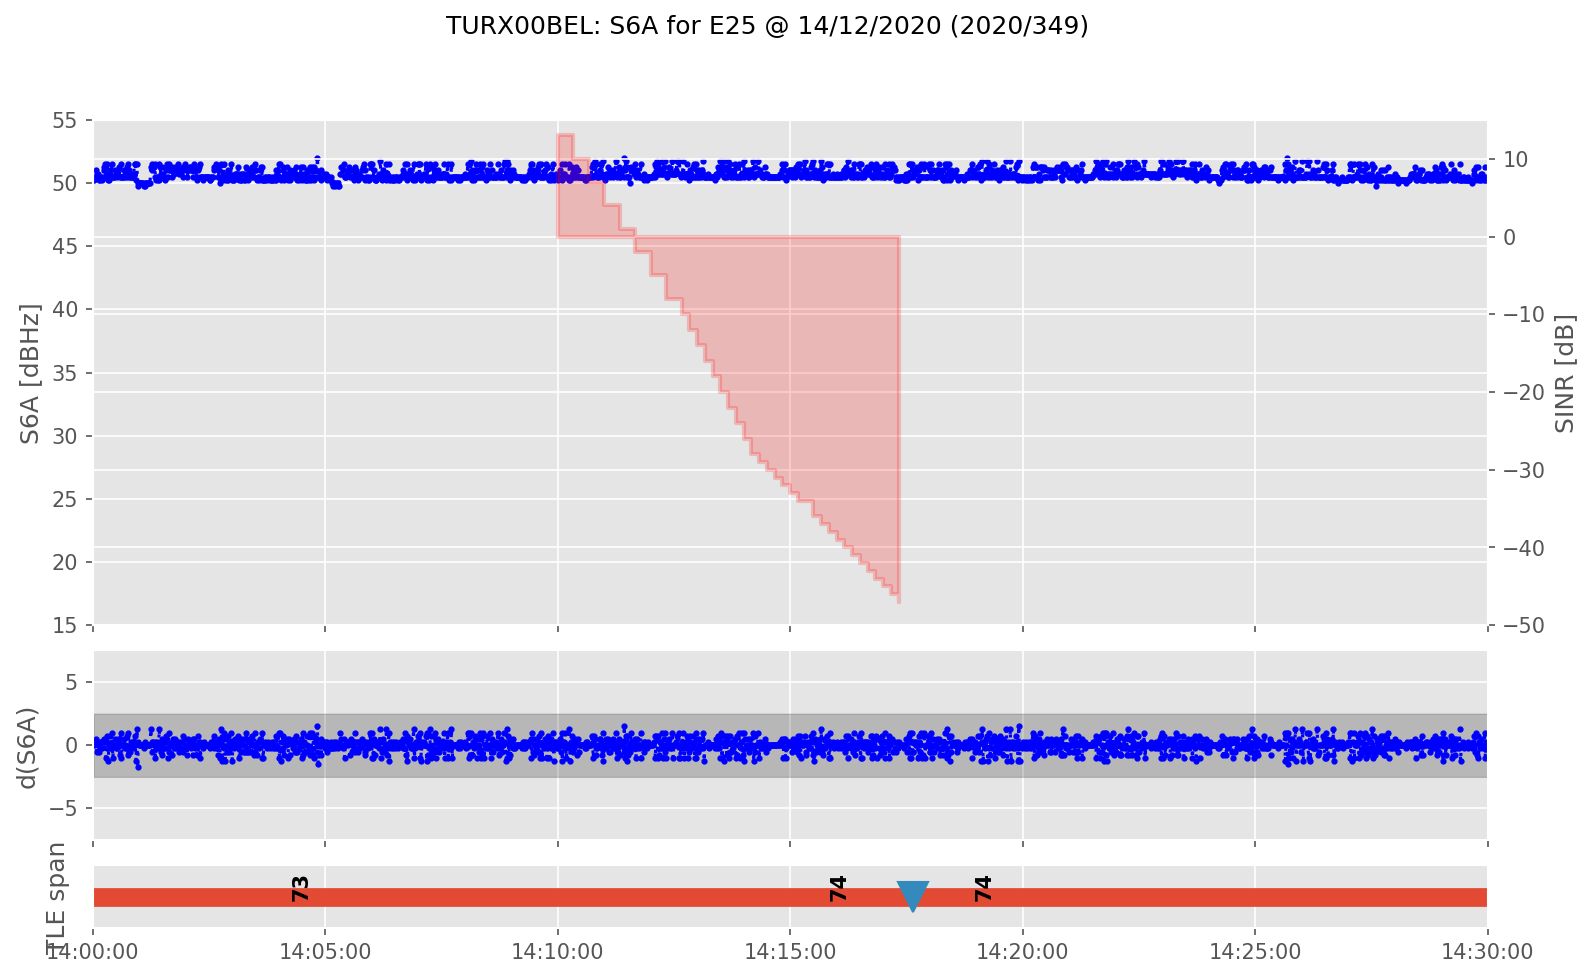
\includegraphics[width=0.95\linewidth]{png/TURX00BEL_R_20203491400_30M_01S_MO_E-S6A-E25.png}%
\end{figure}

%


\begin{figure}[H]%
\centering%
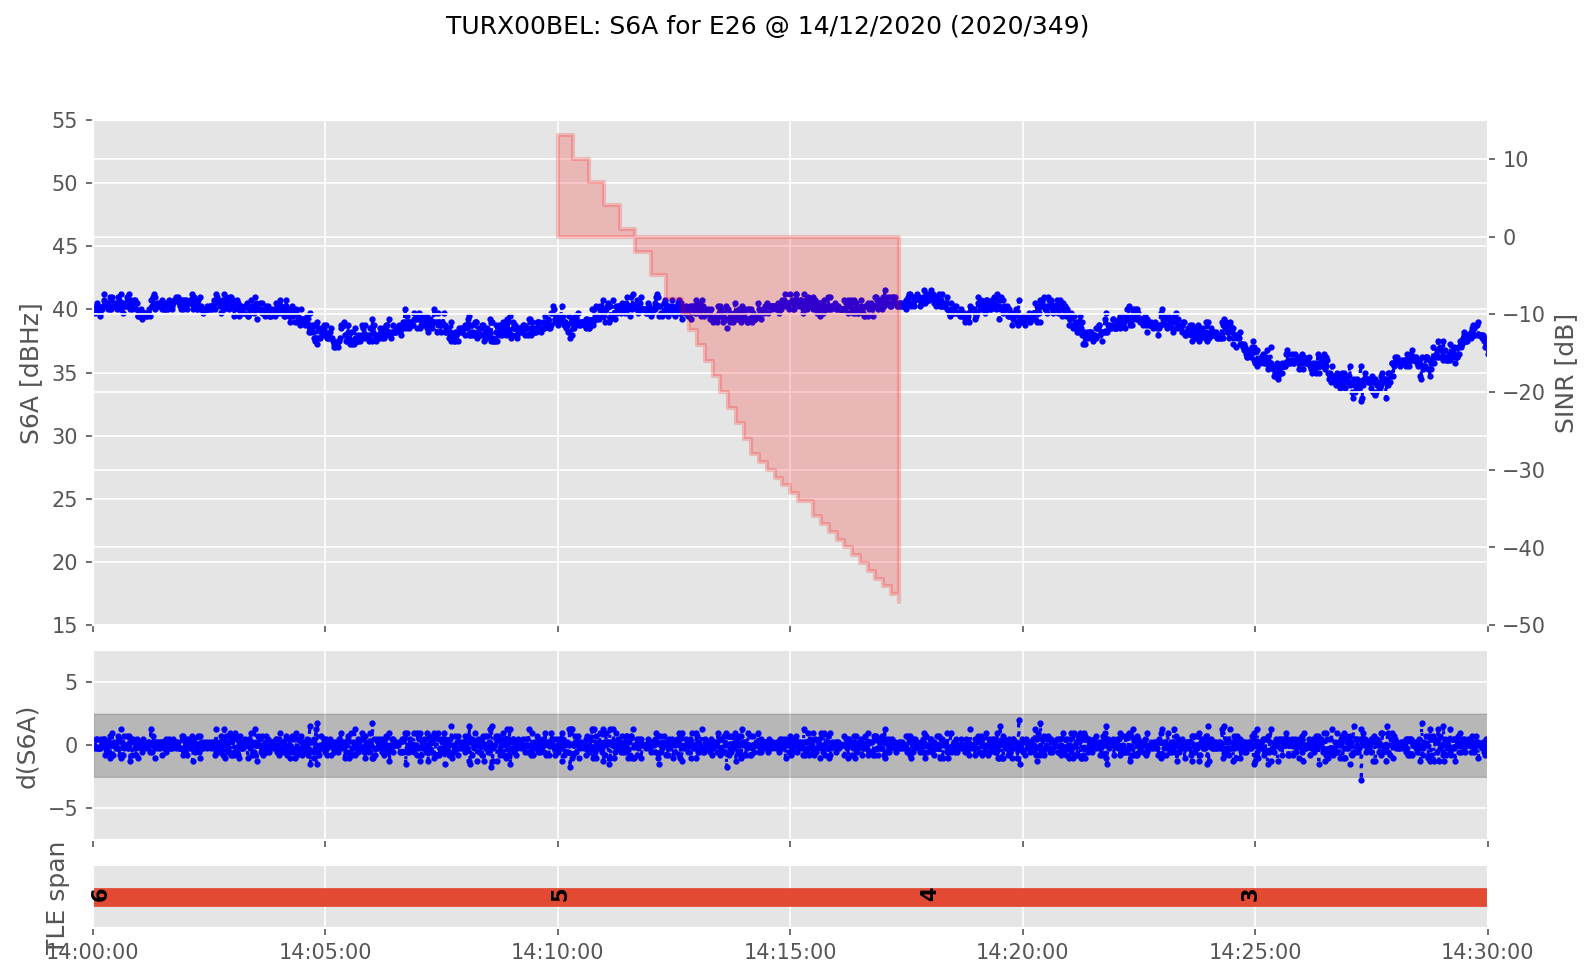
\includegraphics[width=0.95\linewidth]{png/TURX00BEL_R_20203491400_30M_01S_MO_E-S6A-E26.png}%
\end{figure}

%


\begin{figure}[H]%
\centering%
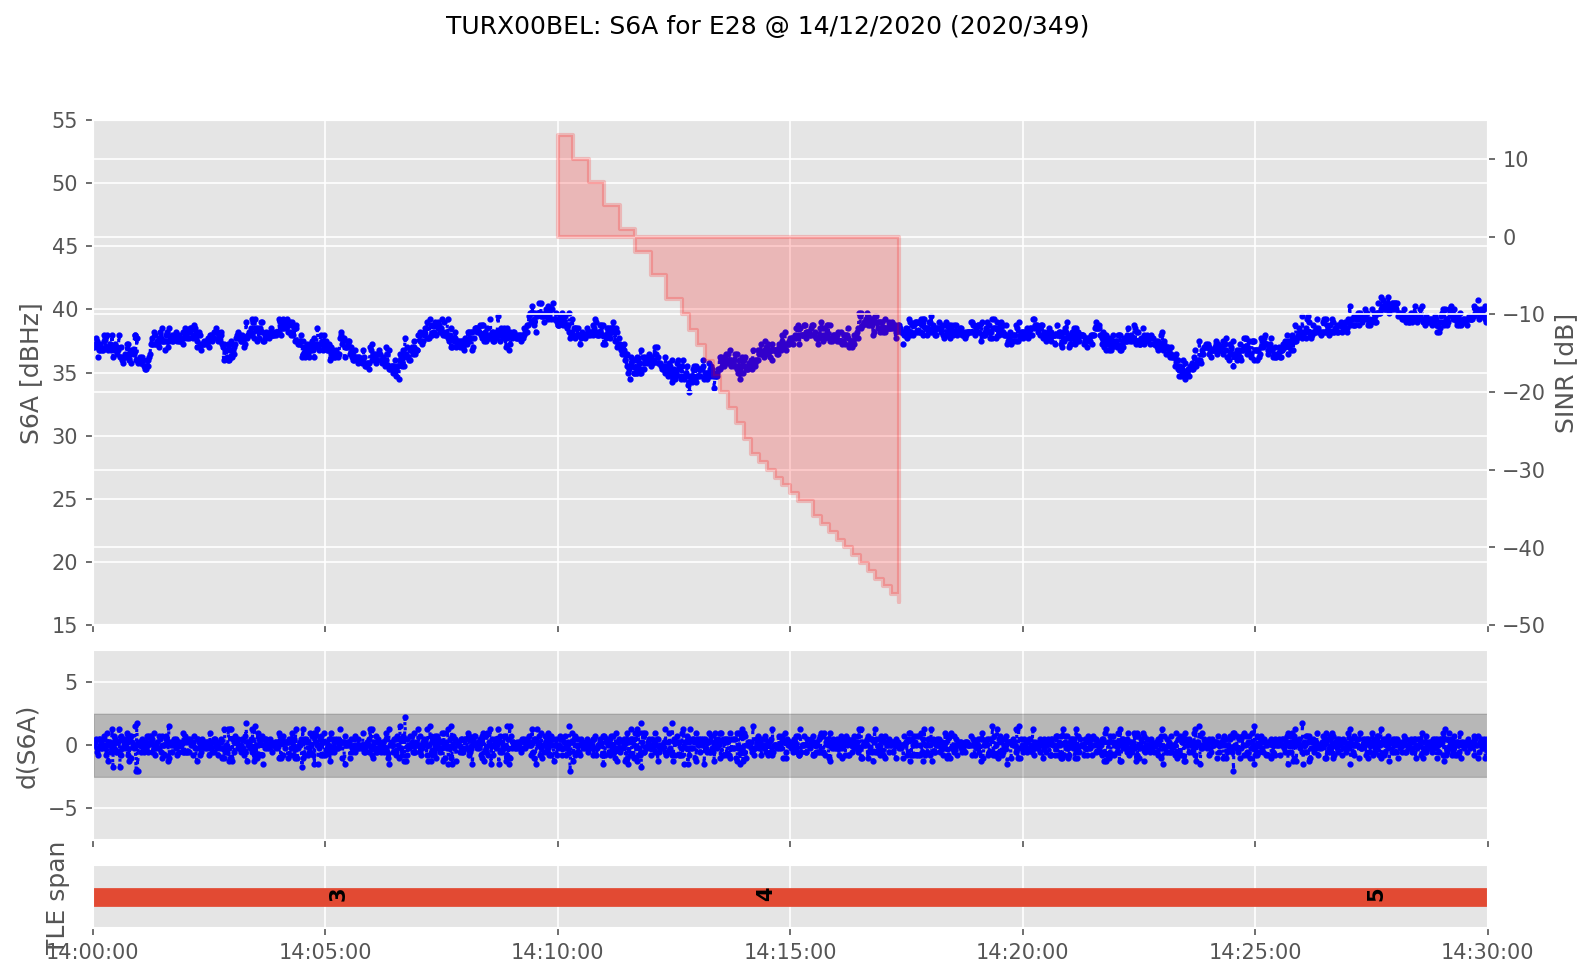
\includegraphics[width=0.95\linewidth]{png/TURX00BEL_R_20203491400_30M_01S_MO_E-S6A-E28.png}%
\end{figure}

%
\end{enumerate}

%
\newpage%
\paragraph{Analysis of navigation signal E1A}%
\label{para:AnalysisofnavigationsignalE1A}%
\newpage%
\begin{enumerate}%
\item%
Figure \ref{fig:tle_navsig_1AE} represents the observed time span for navigation signal E1A set out against the maximum time span calculated from the  Two Line Elements (TLE). If present, the culmination point for a satellite is represented by a triangle. The time span from TLEs is represented by the lighter area while the real observations are represented by the dark super-imposed areas.%


\begin{figure}[H]%
\centering%
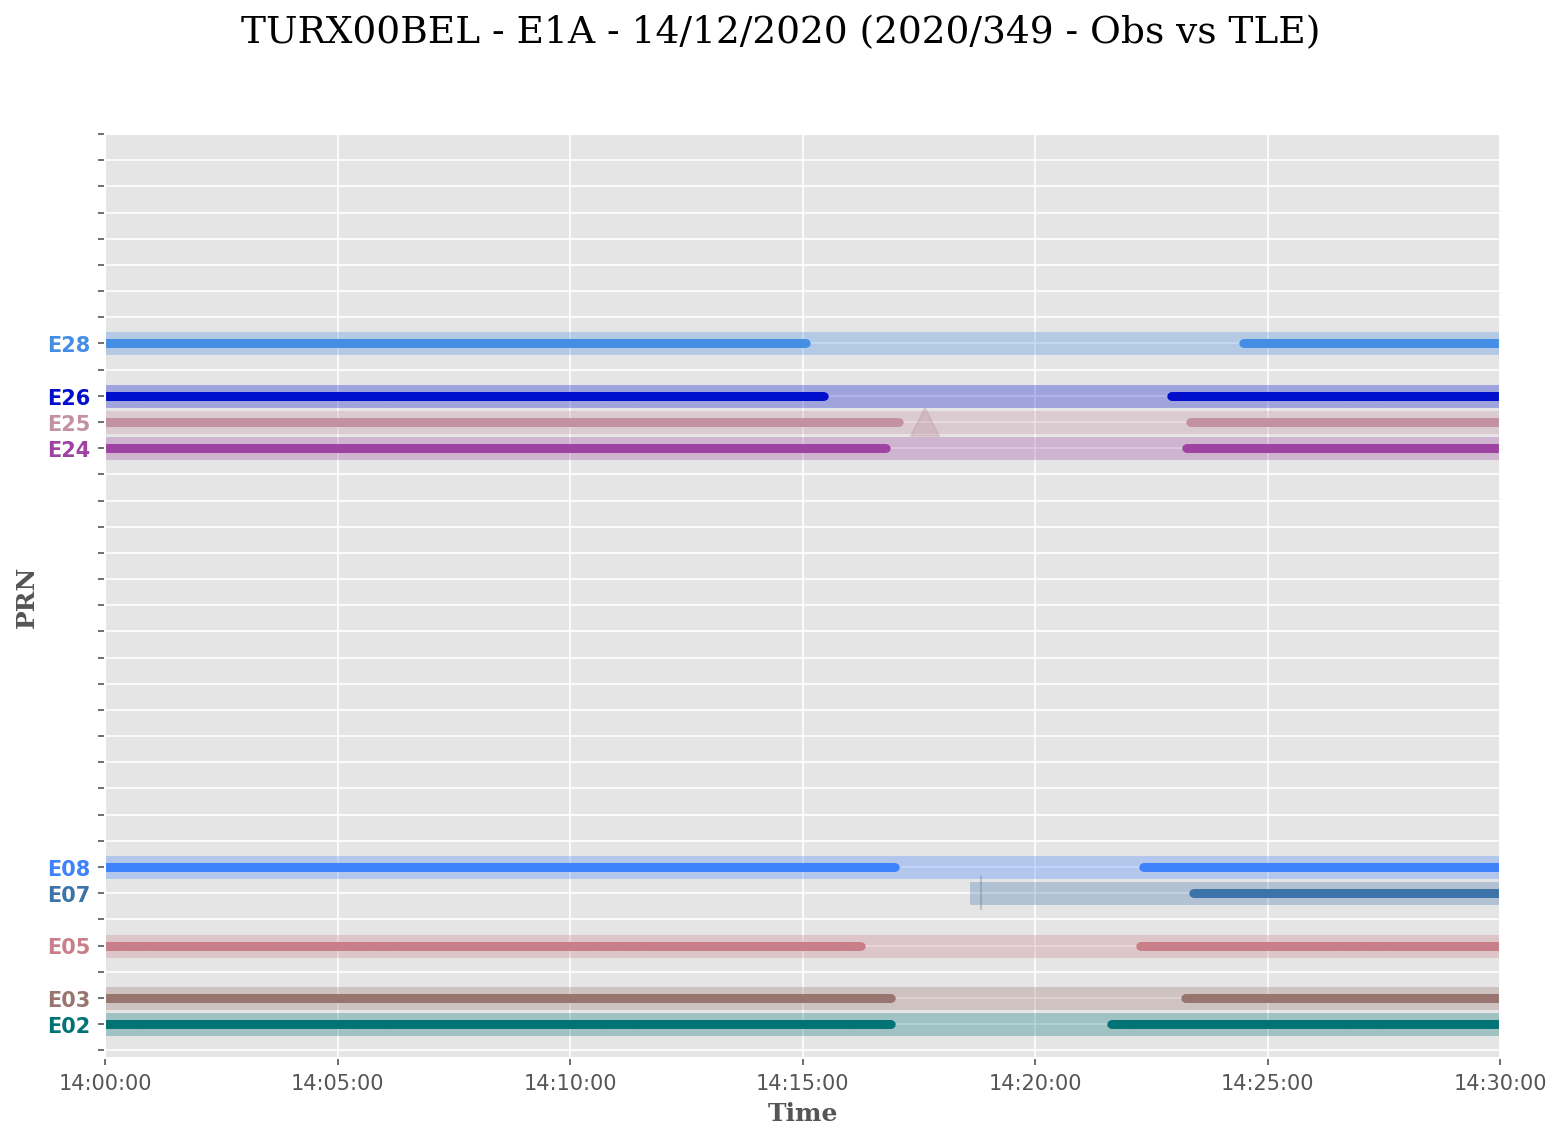
\includegraphics[width=0.95\textwidth]{png/TURX00BEL_R_20203491400_30M_01S_MO_E-E1A-TLE-arcs.png}%
\caption{\label{fig:tle_navsig_1AE} Navigation signal E1A versus TLE time span}%
\end{figure}

%
\item%
Figure \ref{fig:tle_navsig_ES1A} displays the evolution of observation type S1A. \newline The upper plot represents the variation of the observation type while the middle plot (if available) displays the variation of this observable between 2 consecutive epochs. The bottom plot displays the TLE time spans for the satellies.%


\begin{figure}[H]%
\centering%
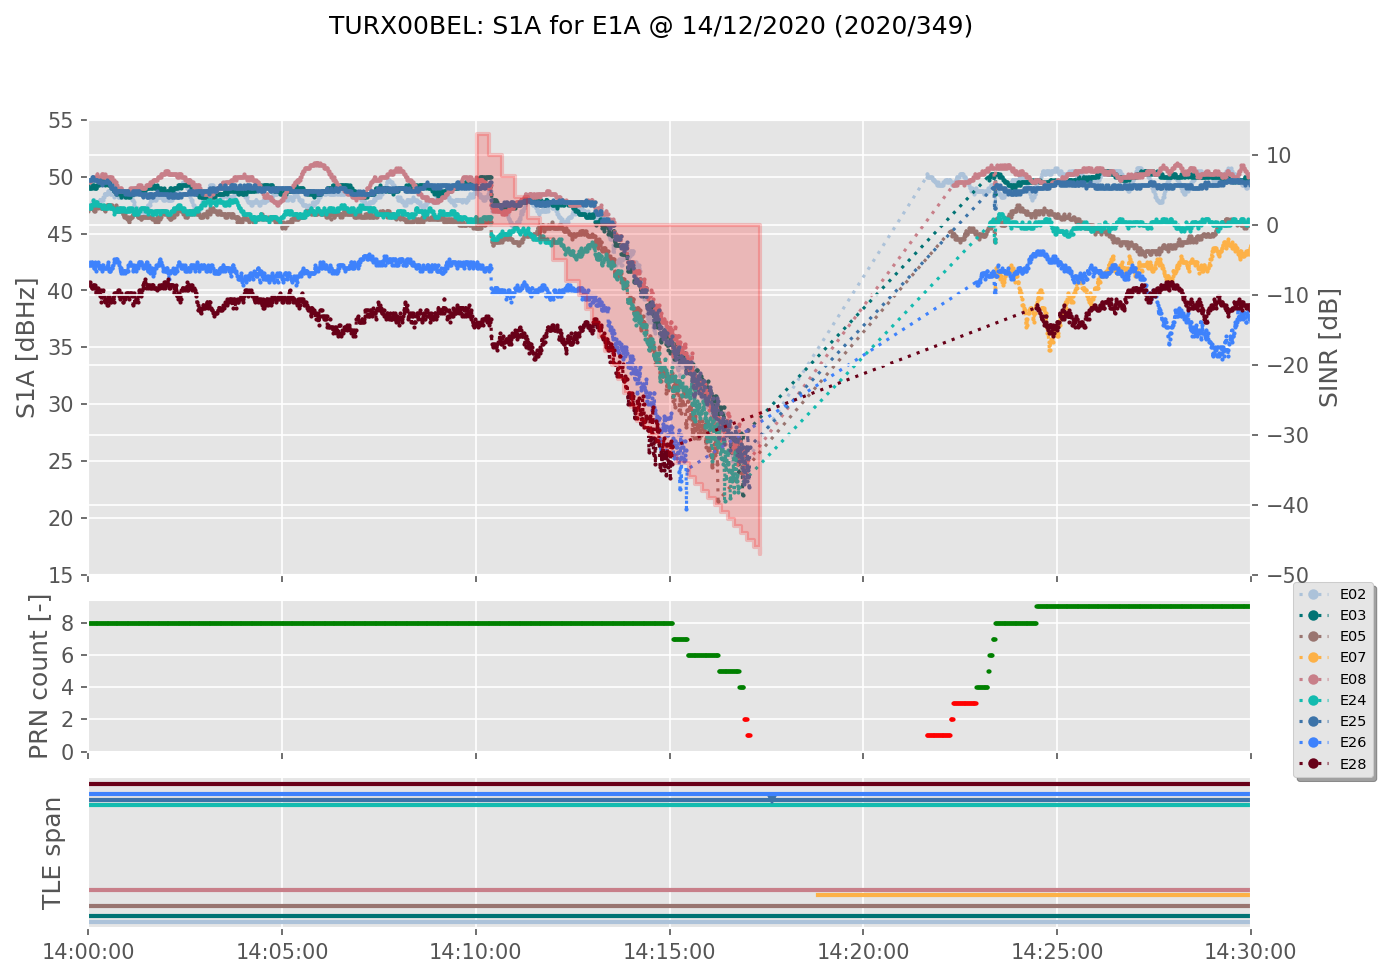
\includegraphics[width=0.95\textwidth]{png/TURX00BEL_R_20203491400_30M_01S_MO_E-E1A-S1A.png}%
\caption{\label{fig:tle_navsig_ES1A} Navigation signal S1A evolution}%
\end{figure}

%
The table below reports the loss and reacquisition of PNT for observable S1A.%
%
\begin{longtabu}{ccccc}%
\hline%
\multicolumn{5}{c}{\textcolor{blue}{%
Navigation signal 1A%
}}\\%
\textbf{DATE\_TIME}&\textbf{event}&\textbf{type}&\textbf{duration}&\textbf{reacq}\\%
\hline%
\endhead%
\hline%
\multicolumn{5}{r}{Continued on Next Page}\\%
\hline%
\endfoot%
\hline%
\endlastfoot%
2020{-}12{-}14 14:16:54&Loss&PNT&361.0&2020{-}12{-}14 14:22:55\\%
\hline%
\end{longtabu}%
\item%
Analysis of navigation signal E1A for each observed satellite.\newline%
ewline The following plots display the same information as described above per satellite. Each plot is accompanied by a table displaying the time of loss of lock and reacquisition of the satellite when such events are detected.%


\begin{figure}[H]%
\centering%
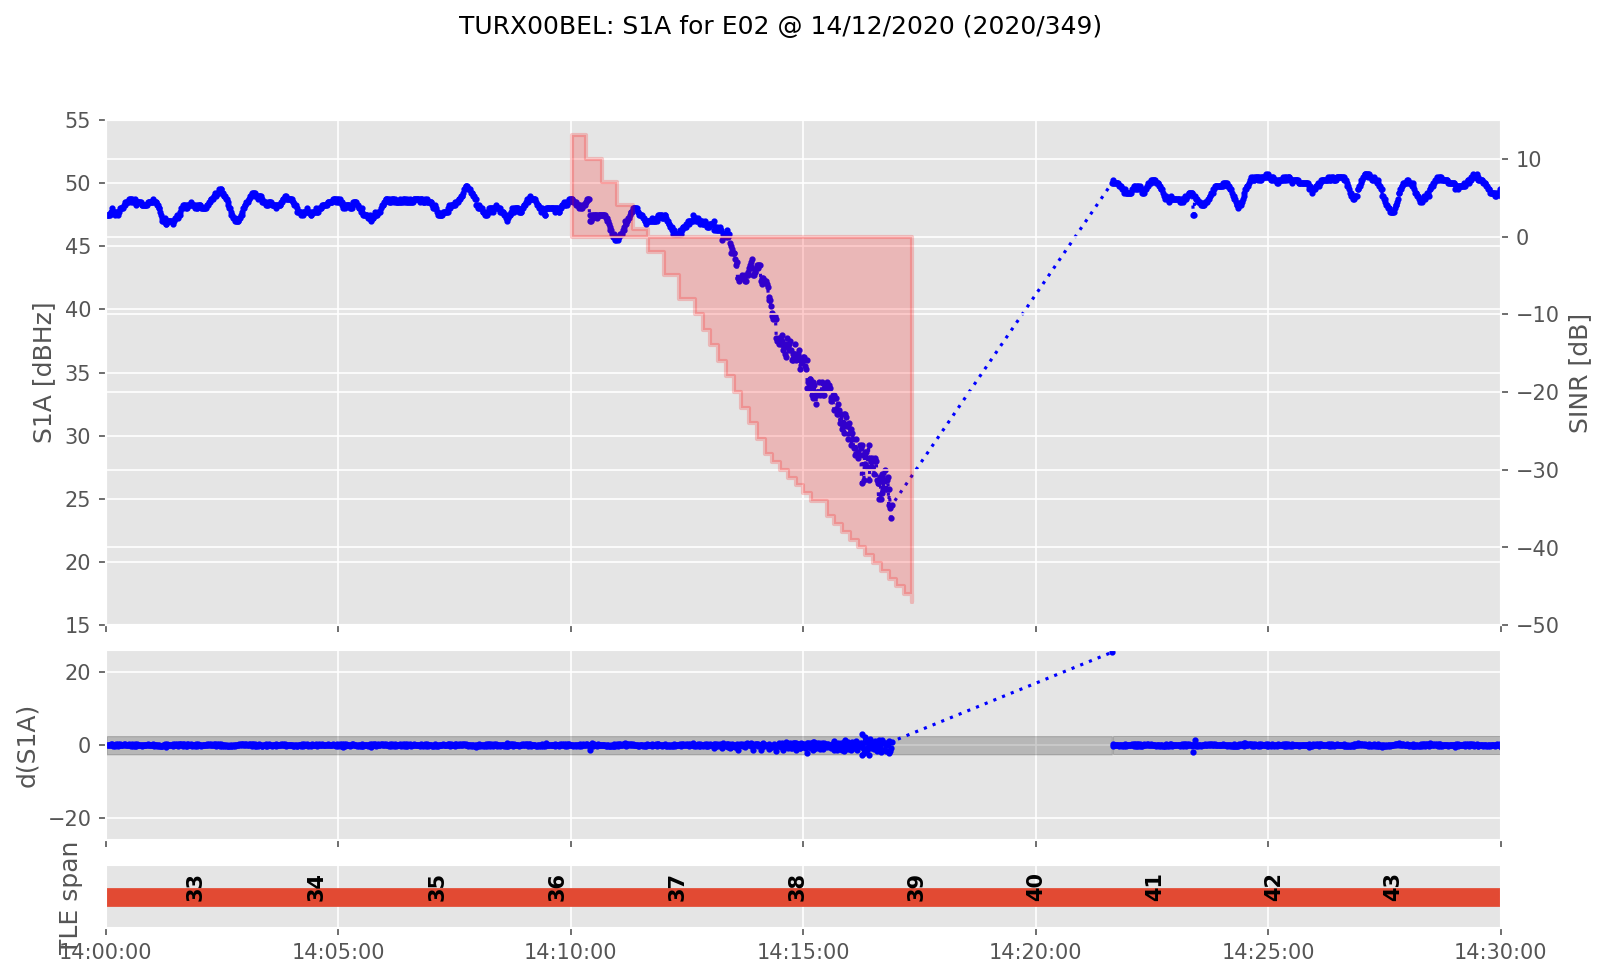
\includegraphics[width=0.95\linewidth]{png/TURX00BEL_R_20203491400_30M_01S_MO_E-S1A-E02.png}%
\end{figure}

%
\begin{longtabu}{ccccc}%
\hline%
\multicolumn{5}{c}{\textcolor{blue}{%
Navigation signal 1A%
}}\\%
\textbf{DATE\_TIME}&\textbf{event}&\textbf{type}&\textbf{duration}&\textbf{reacq}\\%
\hline%
\endhead%
\hline%
\multicolumn{5}{r}{Continued on Next Page}\\%
\hline%
\endfoot%
\hline%
\endlastfoot%
2020{-}12{-}14 14:16:54&Loss&E02&284.0&2020{-}12{-}14 14:21:38\\%
\hline%
\end{longtabu}%


\begin{figure}[H]%
\centering%
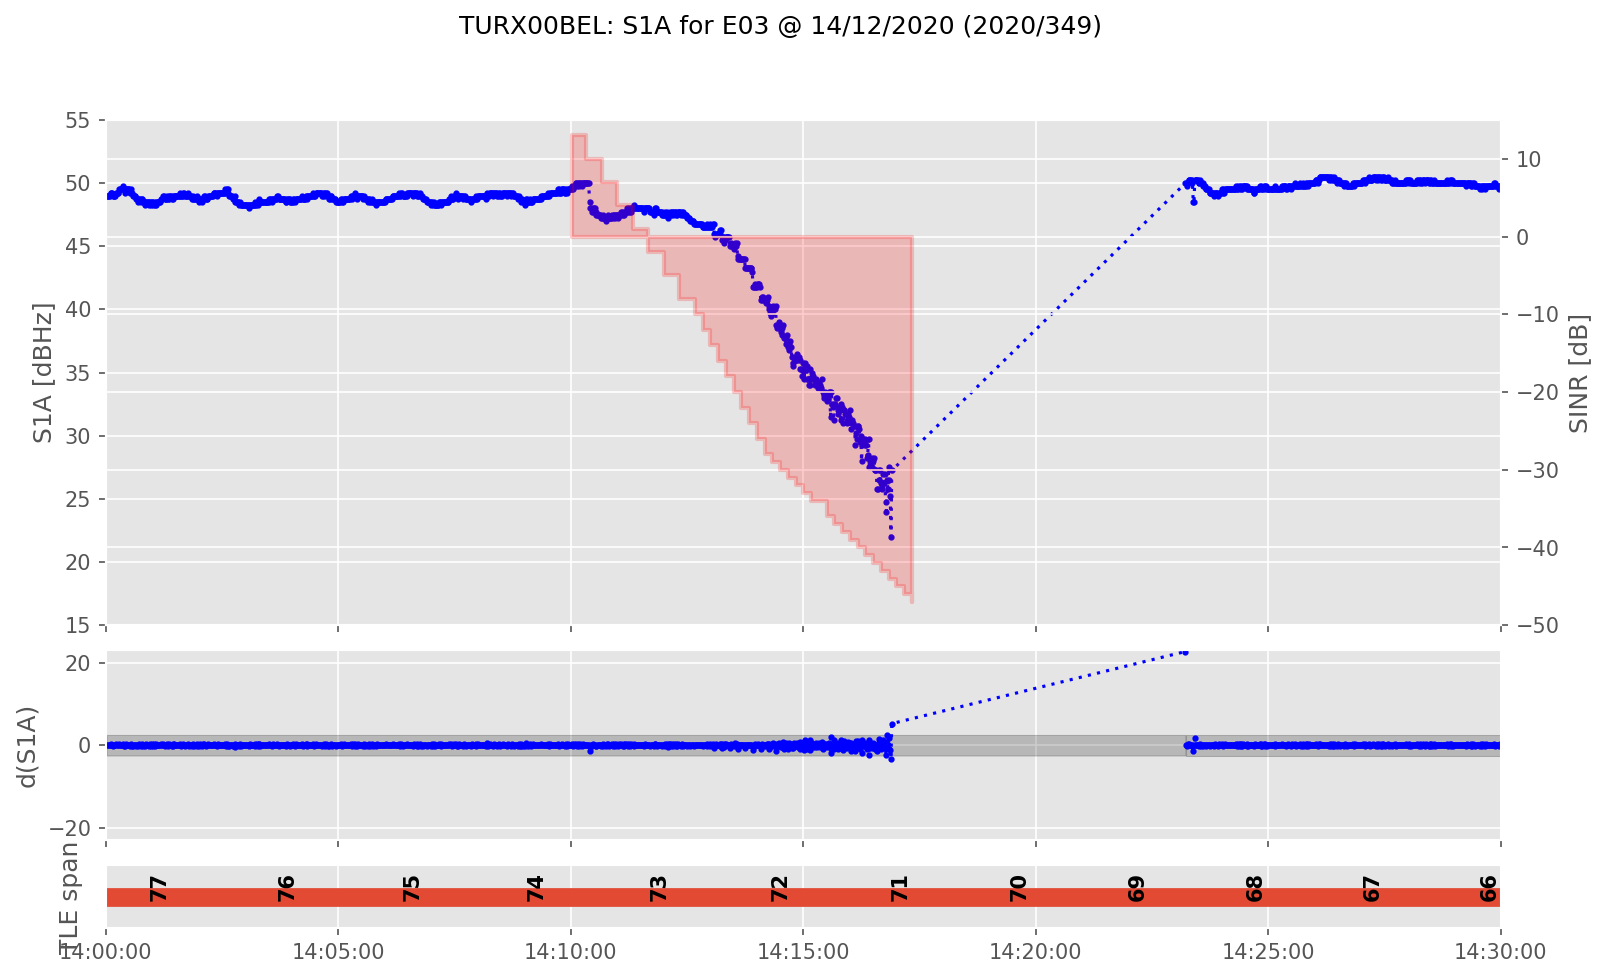
\includegraphics[width=0.95\linewidth]{png/TURX00BEL_R_20203491400_30M_01S_MO_E-S1A-E03.png}%
\end{figure}

%
\begin{longtabu}{ccccc}%
\hline%
\multicolumn{5}{c}{\textcolor{blue}{%
Navigation signal 1A%
}}\\%
\textbf{DATE\_TIME}&\textbf{event}&\textbf{type}&\textbf{duration}&\textbf{reacq}\\%
\hline%
\endhead%
\hline%
\multicolumn{5}{r}{Continued on Next Page}\\%
\hline%
\endfoot%
\hline%
\endlastfoot%
2020{-}12{-}14 14:16:54&Loss&E03&379.0&2020{-}12{-}14 14:23:13\\%
\hline%
\end{longtabu}%


\begin{figure}[H]%
\centering%
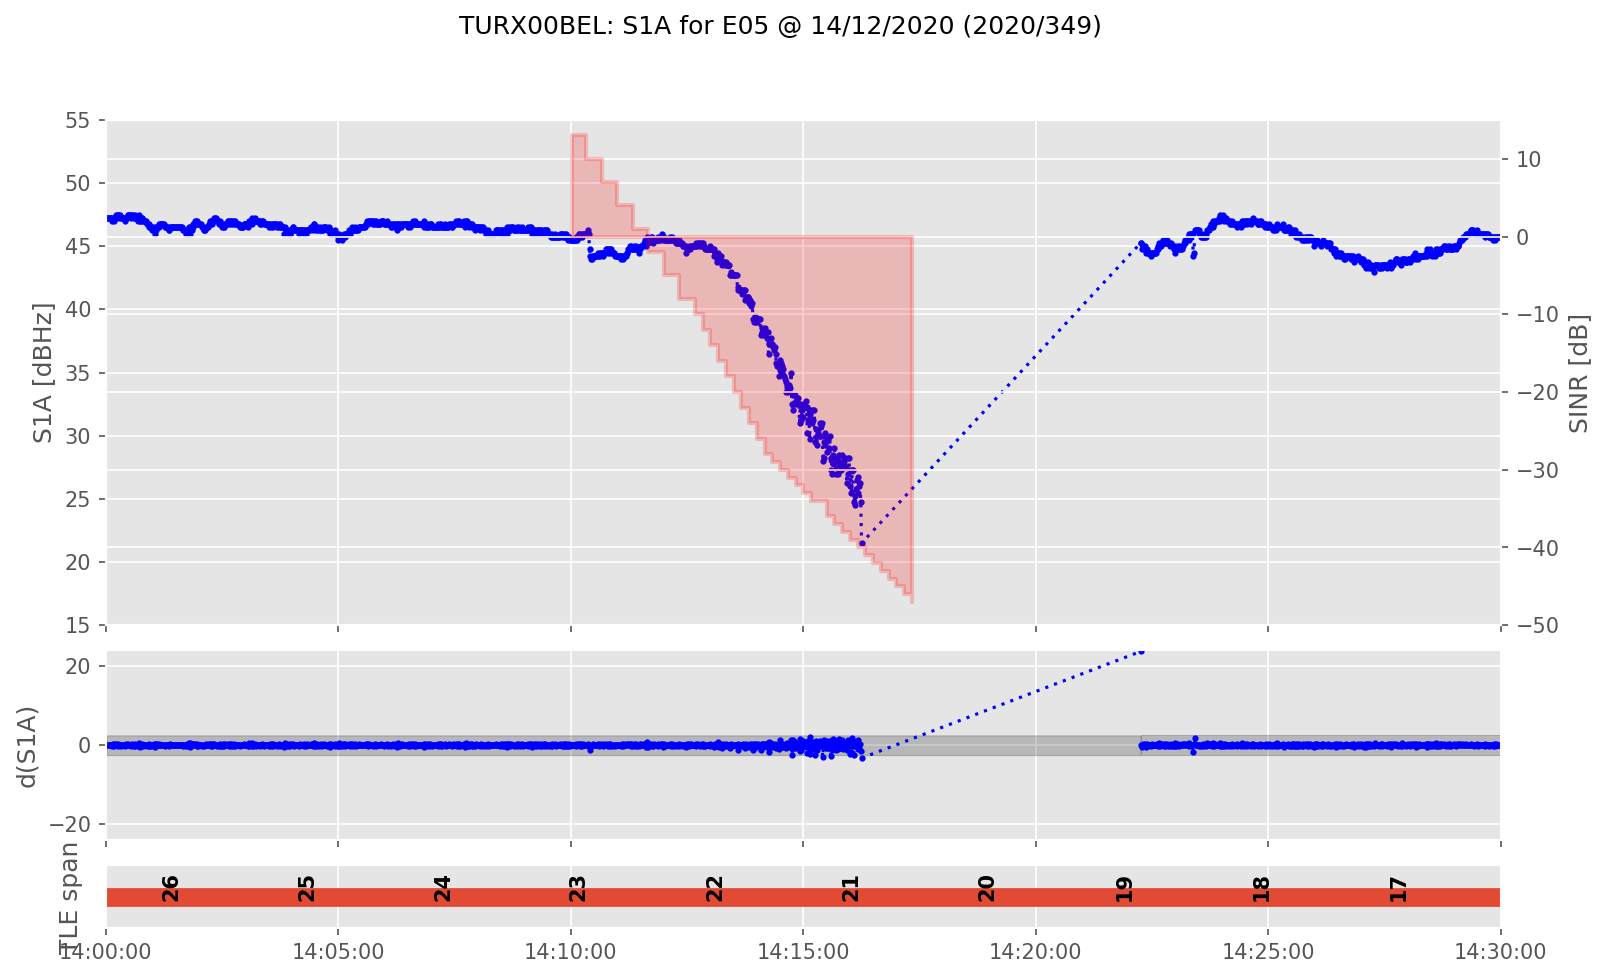
\includegraphics[width=0.95\linewidth]{png/TURX00BEL_R_20203491400_30M_01S_MO_E-S1A-E05.png}%
\end{figure}

%
\begin{longtabu}{ccccc}%
\hline%
\multicolumn{5}{c}{\textcolor{blue}{%
Navigation signal 1A%
}}\\%
\textbf{DATE\_TIME}&\textbf{event}&\textbf{type}&\textbf{duration}&\textbf{reacq}\\%
\hline%
\endhead%
\hline%
\multicolumn{5}{r}{Continued on Next Page}\\%
\hline%
\endfoot%
\hline%
\endlastfoot%
2020{-}12{-}14 14:16:15&Loss&E05&360.0&2020{-}12{-}14 14:22:15\\%
\hline%
\end{longtabu}%


\begin{figure}[H]%
\centering%
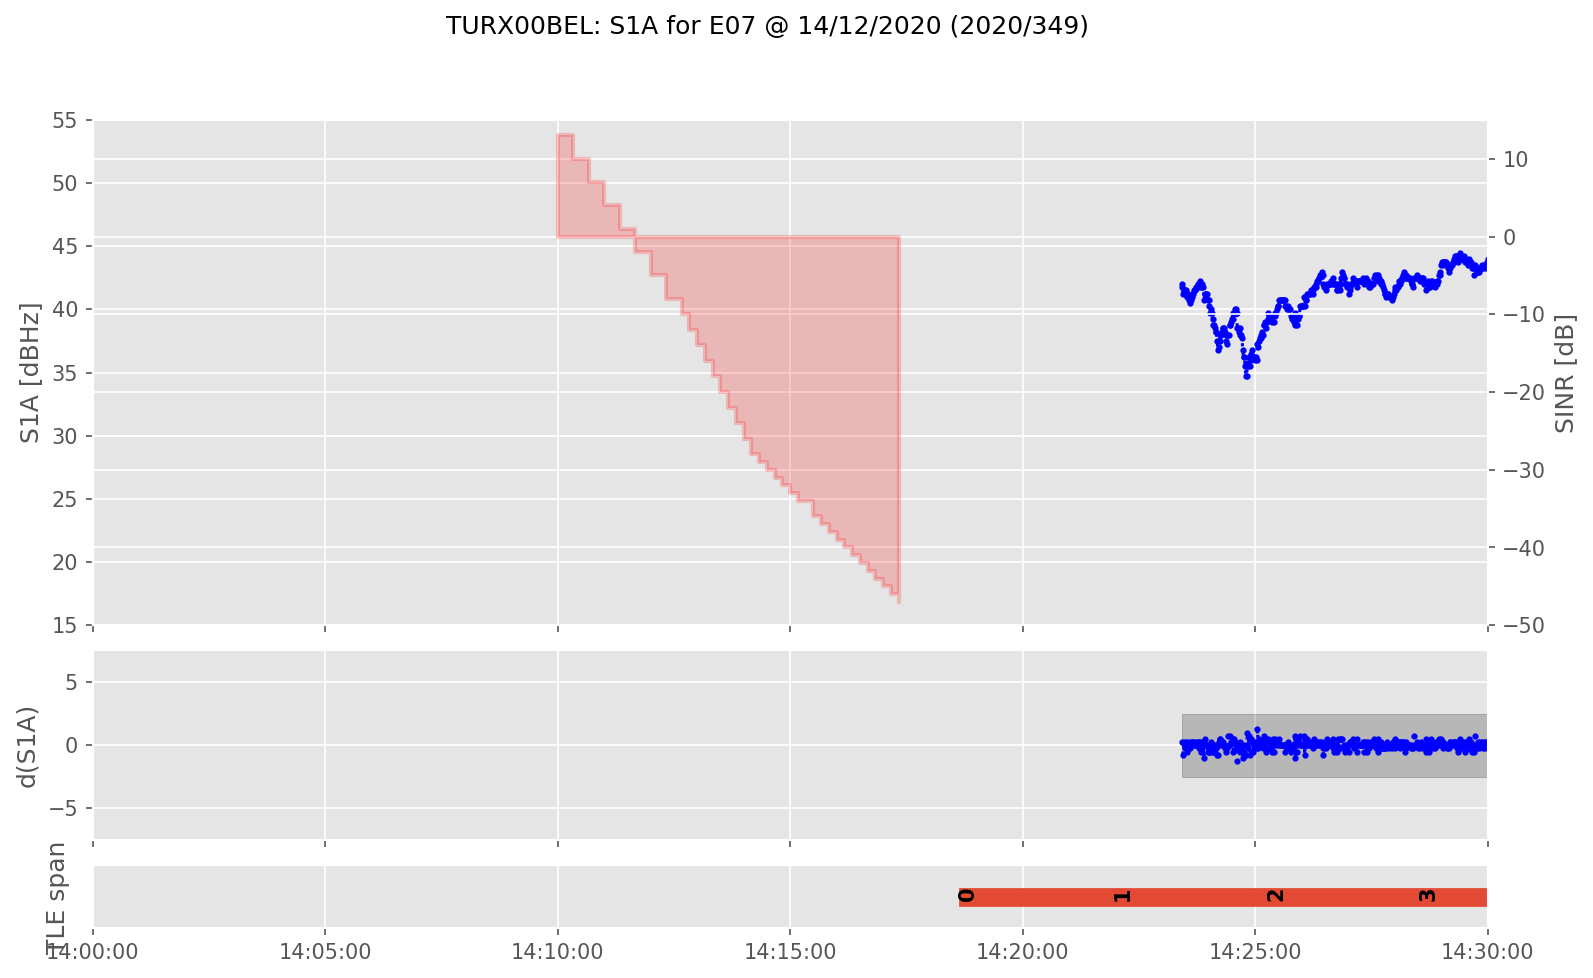
\includegraphics[width=0.95\linewidth]{png/TURX00BEL_R_20203491400_30M_01S_MO_E-S1A-E07.png}%
\end{figure}

%


\begin{figure}[H]%
\centering%
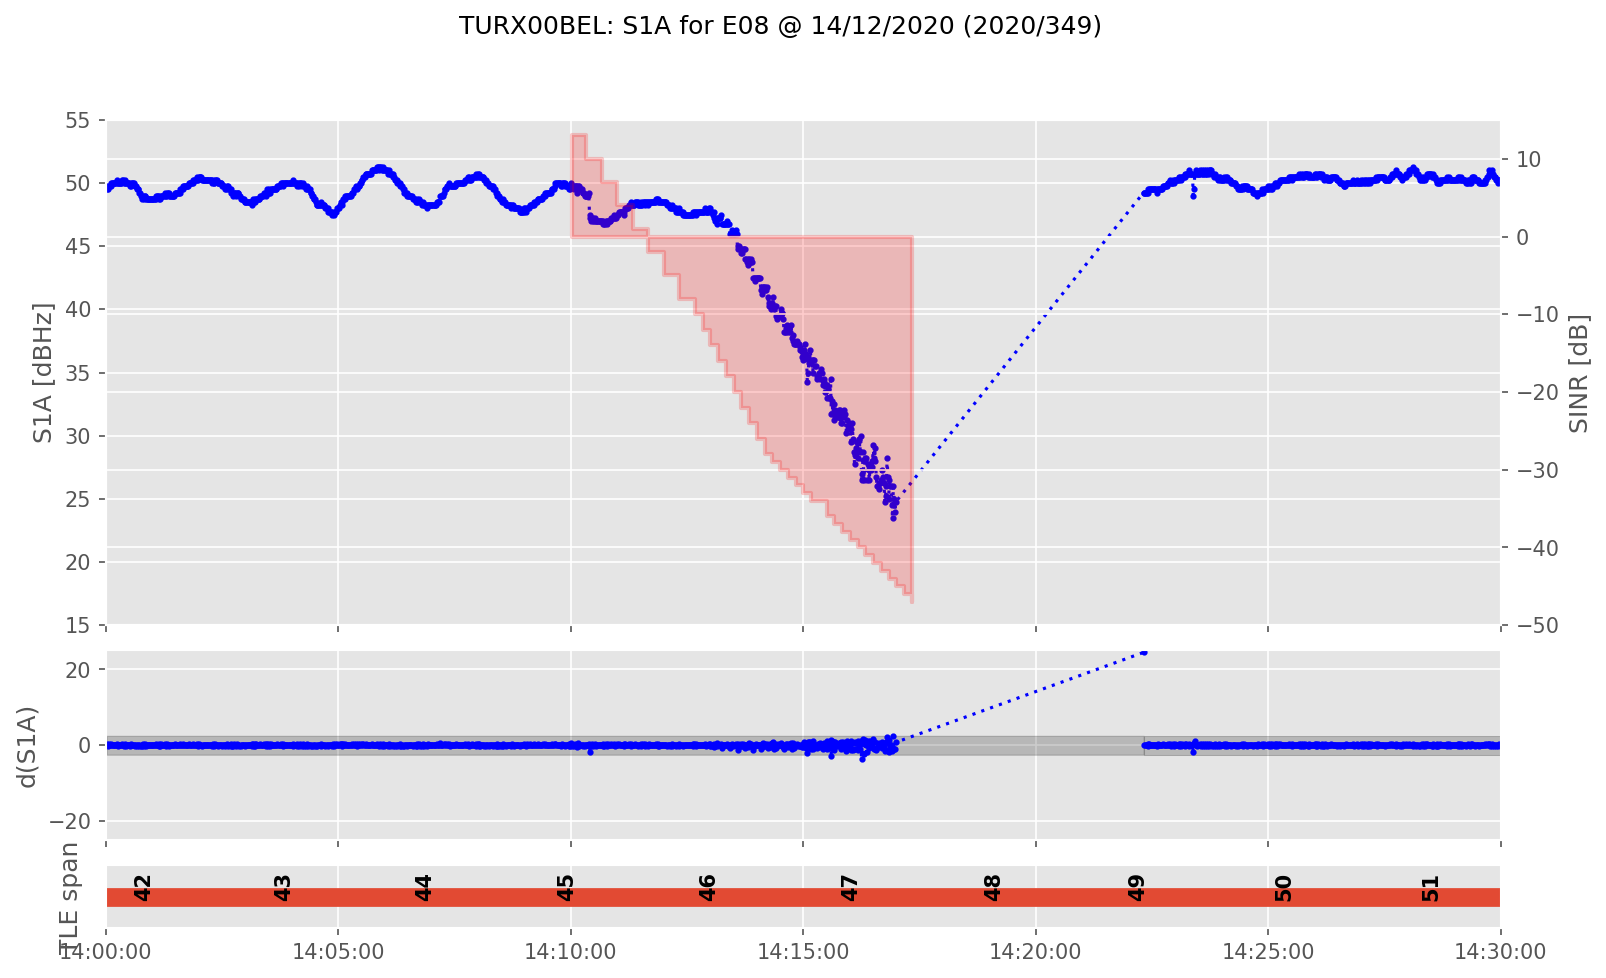
\includegraphics[width=0.95\linewidth]{png/TURX00BEL_R_20203491400_30M_01S_MO_E-S1A-E08.png}%
\end{figure}

%
\begin{longtabu}{ccccc}%
\hline%
\multicolumn{5}{c}{\textcolor{blue}{%
Navigation signal 1A%
}}\\%
\textbf{DATE\_TIME}&\textbf{event}&\textbf{type}&\textbf{duration}&\textbf{reacq}\\%
\hline%
\endhead%
\hline%
\multicolumn{5}{r}{Continued on Next Page}\\%
\hline%
\endfoot%
\hline%
\endlastfoot%
2020{-}12{-}14 14:16:59&Loss&E08&320.0&2020{-}12{-}14 14:22:19\\%
\hline%
\end{longtabu}%


\begin{figure}[H]%
\centering%
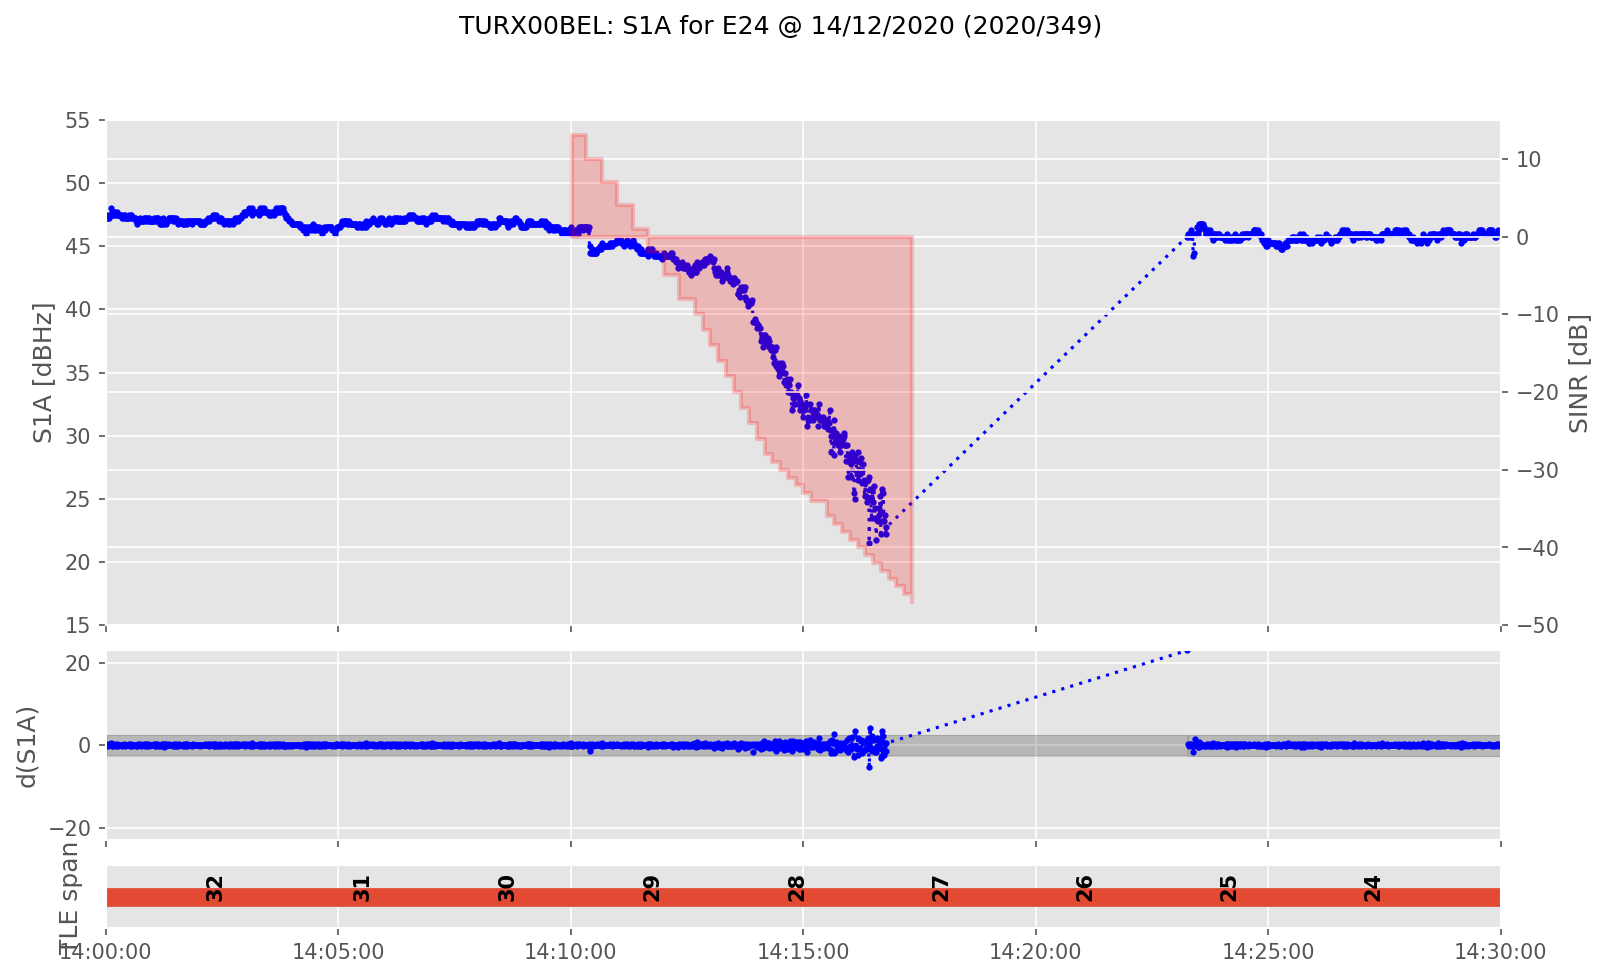
\includegraphics[width=0.95\linewidth]{png/TURX00BEL_R_20203491400_30M_01S_MO_E-S1A-E24.png}%
\end{figure}

%
\begin{longtabu}{ccccc}%
\hline%
\multicolumn{5}{c}{\textcolor{blue}{%
Navigation signal 1A%
}}\\%
\textbf{DATE\_TIME}&\textbf{event}&\textbf{type}&\textbf{duration}&\textbf{reacq}\\%
\hline%
\endhead%
\hline%
\multicolumn{5}{r}{Continued on Next Page}\\%
\hline%
\endfoot%
\hline%
\endlastfoot%
2020{-}12{-}14 14:16:47&Loss&E24&388.0&2020{-}12{-}14 14:23:15\\%
\hline%
\end{longtabu}%


\begin{figure}[H]%
\centering%
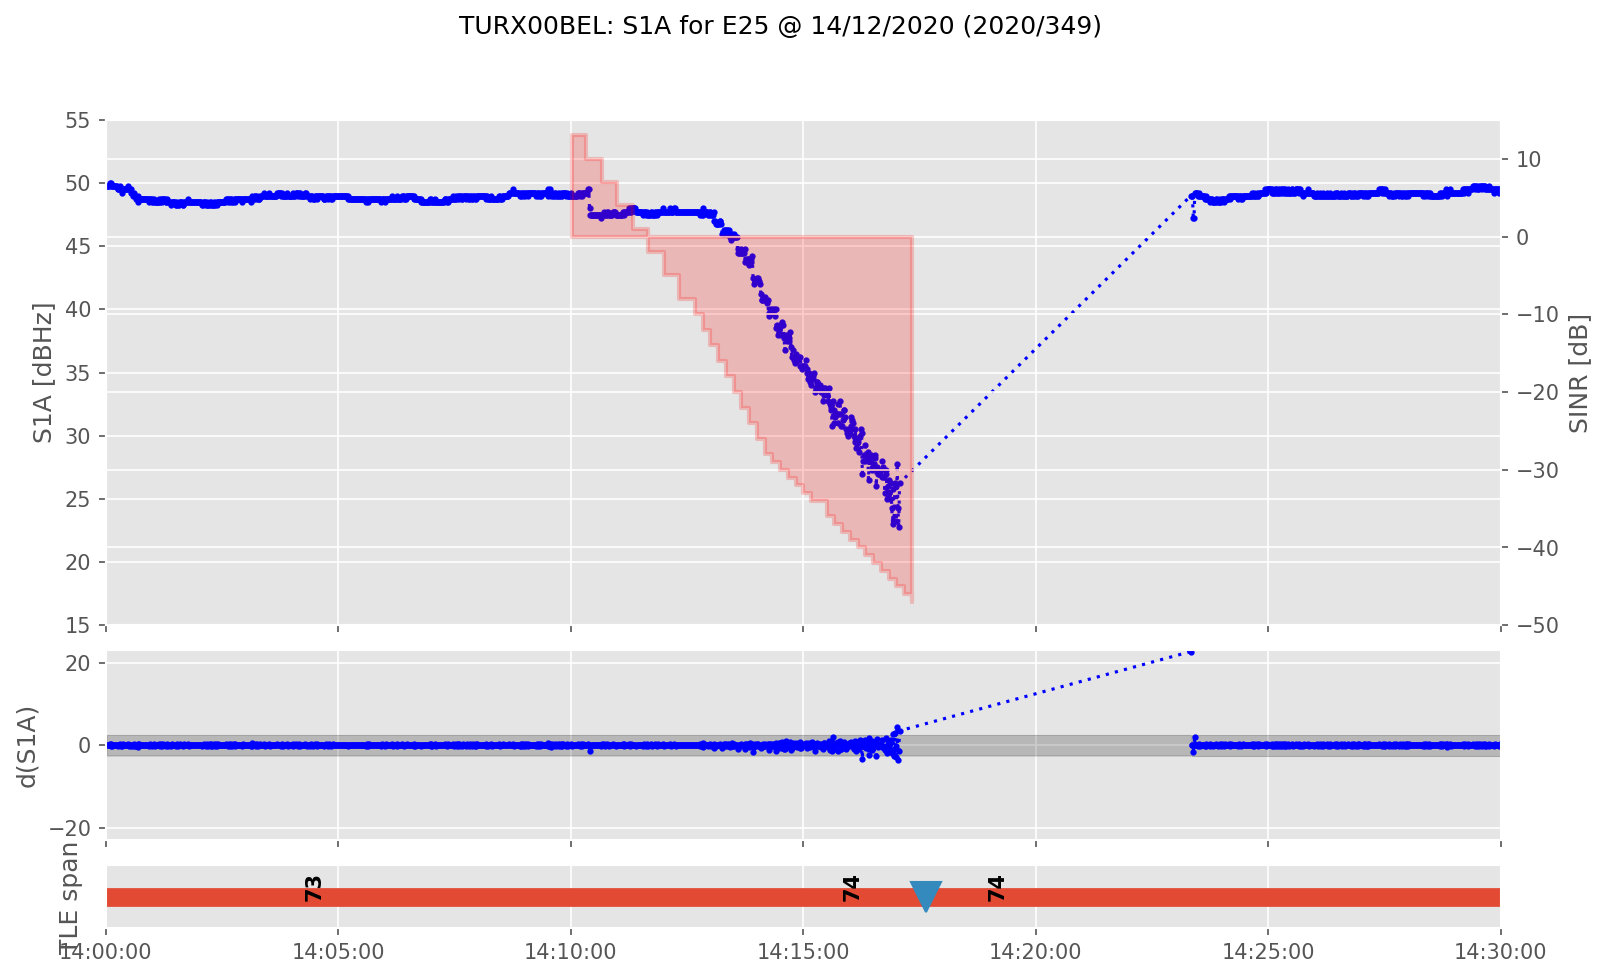
\includegraphics[width=0.95\linewidth]{png/TURX00BEL_R_20203491400_30M_01S_MO_E-S1A-E25.png}%
\end{figure}

%
\begin{longtabu}{ccccc}%
\hline%
\multicolumn{5}{c}{\textcolor{blue}{%
Navigation signal 1A%
}}\\%
\textbf{DATE\_TIME}&\textbf{event}&\textbf{type}&\textbf{duration}&\textbf{reacq}\\%
\hline%
\endhead%
\hline%
\multicolumn{5}{r}{Continued on Next Page}\\%
\hline%
\endfoot%
\hline%
\endlastfoot%
2020{-}12{-}14 14:17:04&Loss&E25&376.0&2020{-}12{-}14 14:23:20\\%
\hline%
\end{longtabu}%


\begin{figure}[H]%
\centering%
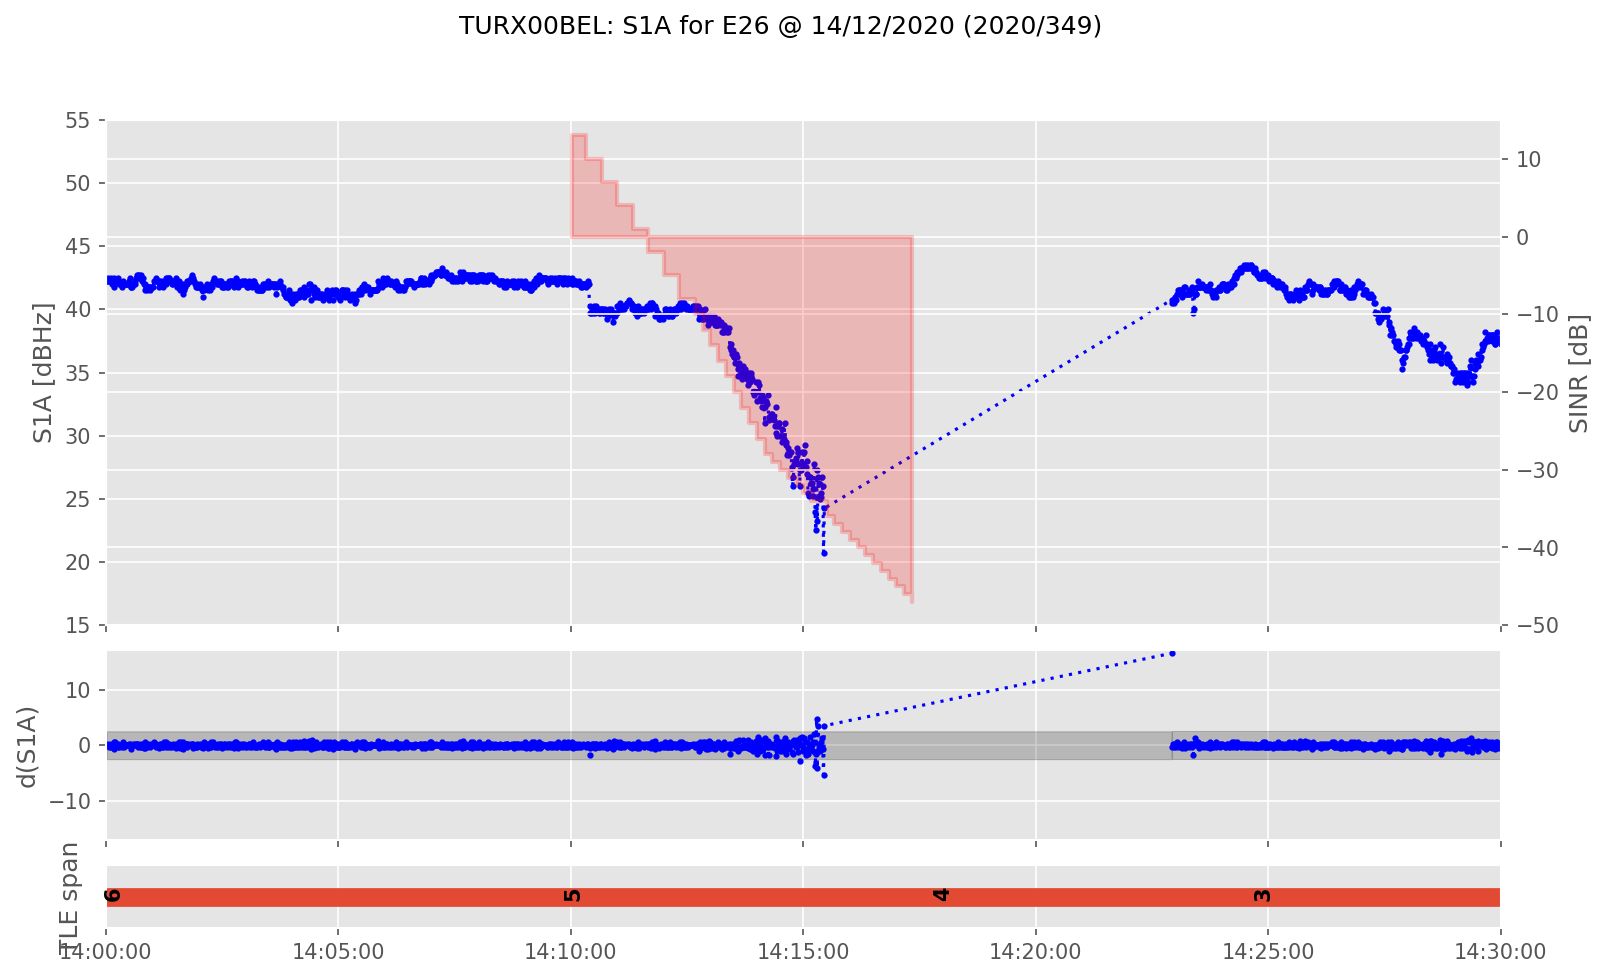
\includegraphics[width=0.95\linewidth]{png/TURX00BEL_R_20203491400_30M_01S_MO_E-S1A-E26.png}%
\end{figure}

%
\begin{longtabu}{ccccc}%
\hline%
\multicolumn{5}{c}{\textcolor{blue}{%
Navigation signal 1A%
}}\\%
\textbf{DATE\_TIME}&\textbf{event}&\textbf{type}&\textbf{duration}&\textbf{reacq}\\%
\hline%
\endhead%
\hline%
\multicolumn{5}{r}{Continued on Next Page}\\%
\hline%
\endfoot%
\hline%
\endlastfoot%
2020{-}12{-}14 14:15:27&Loss&E26&448.0&2020{-}12{-}14 14:22:55\\%
\hline%
\end{longtabu}%


\begin{figure}[H]%
\centering%
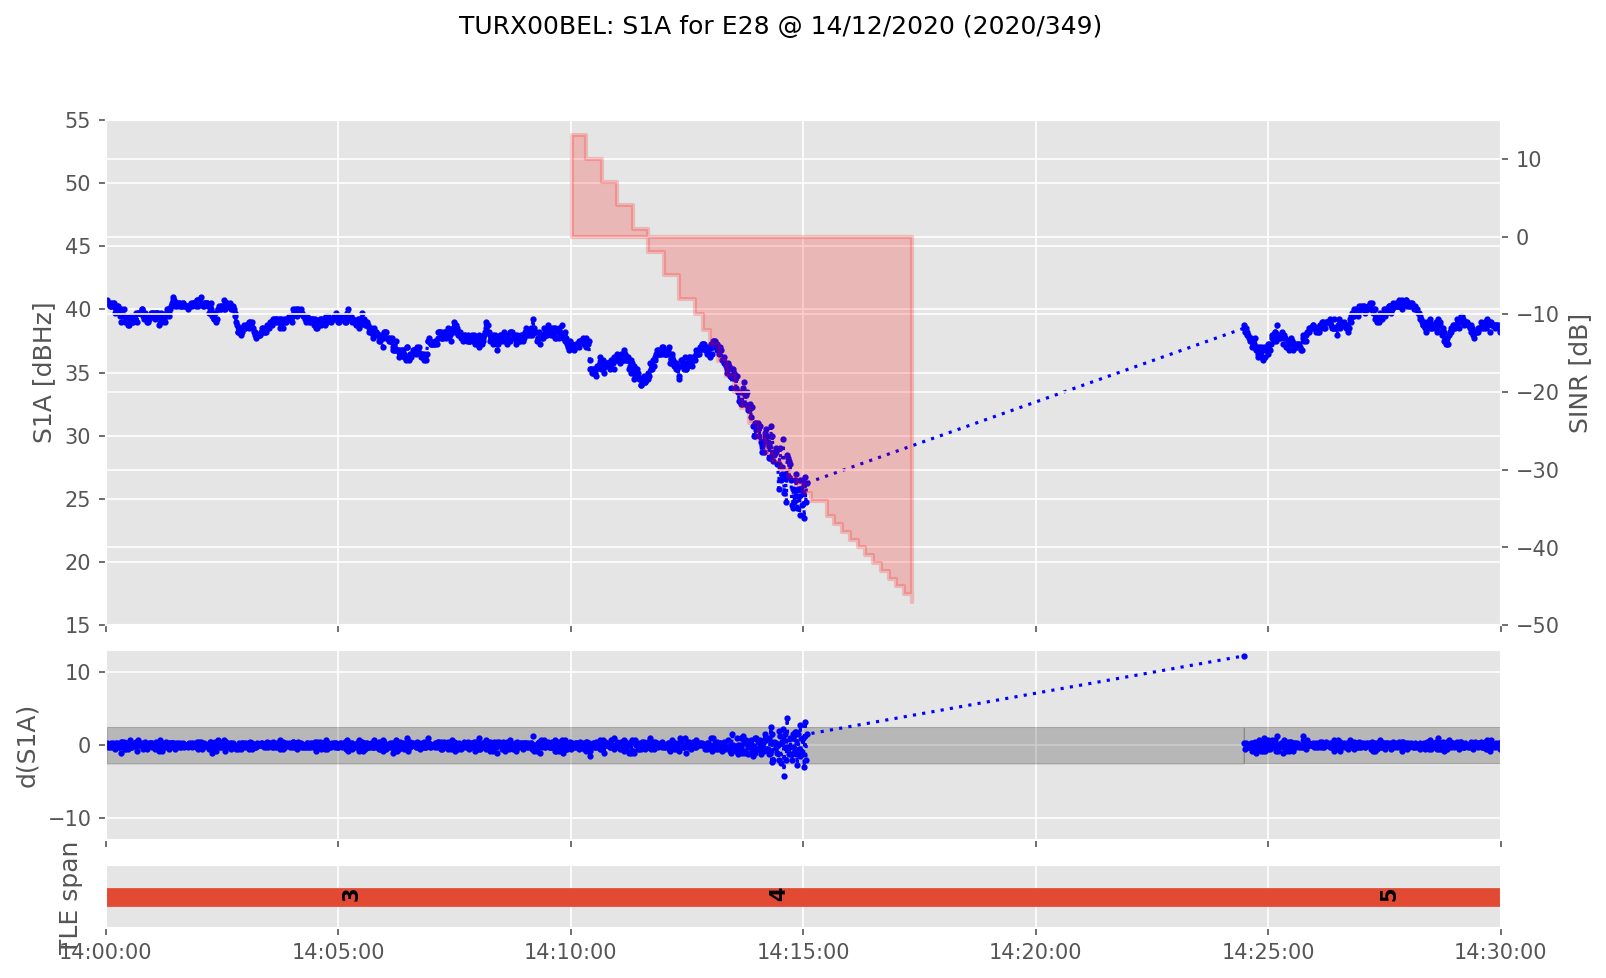
\includegraphics[width=0.95\linewidth]{png/TURX00BEL_R_20203491400_30M_01S_MO_E-S1A-E28.png}%
\end{figure}

%
\begin{longtabu}{ccccc}%
\hline%
\multicolumn{5}{c}{\textcolor{blue}{%
Navigation signal 1A%
}}\\%
\textbf{DATE\_TIME}&\textbf{event}&\textbf{type}&\textbf{duration}&\textbf{reacq}\\%
\hline%
\endhead%
\hline%
\multicolumn{5}{r}{Continued on Next Page}\\%
\hline%
\endfoot%
\hline%
\endlastfoot%
2020{-}12{-}14 14:15:04&Loss&E28&564.0&2020{-}12{-}14 14:24:28\\%
\hline%
\end{longtabu}%
\item%
Chronological overview of detected events for navigation signal E1A%
\begin{longtabu}{cccc}%
\hline%
\multicolumn{4}{c}{\textcolor{blue}{%
Navigation signal 1A%
}}\\%
\textbf{DATE\_TIME}&\textbf{event}&\textbf{type}&\textbf{duration}\\%
\hline%
\endhead%
\hline%
\multicolumn{4}{r}{Continued on Next Page}\\%
\hline%
\endfoot%
\hline%
\endlastfoot%
2020{-}12{-}14 14:15:04&Loss&E28&564.0\\%
2020{-}12{-}14 14:15:27&Loss&E26&448.0\\%
2020{-}12{-}14 14:16:15&Loss&E05&360.0\\%
2020{-}12{-}14 14:16:47&Loss&E24&388.0\\%
2020{-}12{-}14 14:16:54&Loss&PNT&361.0\\%
2020{-}12{-}14 14:16:54&Loss&E02&284.0\\%
2020{-}12{-}14 14:16:54&Loss&E03&379.0\\%
2020{-}12{-}14 14:16:59&Loss&E08&320.0\\%
2020{-}12{-}14 14:17:04&Loss&E25&376.0\\%
2020{-}12{-}14 14:21:38&Reacquisition&E02&nan\\%
2020{-}12{-}14 14:22:15&Reacquisition&E05&nan\\%
2020{-}12{-}14 14:22:19&Reacquisition&E08&nan\\%
2020{-}12{-}14 14:22:55&Reacquisition&PNT&nan\\%
2020{-}12{-}14 14:22:55&Reacquisition&E26&nan\\%
2020{-}12{-}14 14:23:13&Reacquisition&E03&nan\\%
2020{-}12{-}14 14:23:15&Reacquisition&E24&nan\\%
2020{-}12{-}14 14:23:20&Reacquisition&E25&nan\\%
2020{-}12{-}14 14:24:28&Reacquisition&E28&nan\\%
\hline%
\end{longtabu}%
\end{enumerate}

